%--------------------------------------------------------------------------------------------------%
%   Version:    1.0
%   Last Mod:   20170307    
%         By:   Juan Medina juancamilomedina1989@gmail.com
%   Author:     Juan Medina juancamilomedina1989@gmail.com
%--------------------------------------------------------------------------------------------------%

%-------------------------------------------- PREAMBLE --------------------------------------------%
\documentclass[12pt,twoside]{report}
\usepackage[a4paper,width=150mm,headheight=110pt,top=25mm,bottom=25mm]{geometry}
\usepackage[utf8]{inputenc}
\usepackage{listings}
\usepackage{graphicx}
\usepackage{pgffor} 
\usepackage{float}
\usepackage{graphics} 
\usepackage{fancyhdr}
\usepackage{booktabs}
\usepackage{array}
\usepackage{amsmath}
\usepackage{rotating}


\graphicspath{{Images/}}

\usepackage[round, numbers,authoryear]{natbib}
\usepackage{color}
\usepackage[dvipsnames]{xcolor}

\definecolor{mycolor}{RGB}{30,75,180}
\definecolor{mycolor2}{RGB}{40,75,90}
% Lund colors
\definecolor{LUGreen}{RGB}{173,202,184}
\definecolor{LUPink}{RGB}{233,196,199}
\definecolor{LUBlue}{RGB}{0,0,128}
\definecolor{LUBronze}{RGB}{156,97,20}
\definecolor{LUblue}{RGB}{185,211,220}
\definecolor{LUGrey}{RGB}{77,76,68}

\usepackage[colorlinks = true,
            linkcolor = mycolor,
            urlcolor  = mycolor,
            citecolor = mycolor,
            anchorcolor = mycolor]{hyperref}

\usepackage[hypcap=true,font={small,it}]{caption}

\captionsetup{belowskip=2pt,aboveskip=2pt}

\bibliographystyle{apa}
\newtheorem{nullhypothesis}{Null Hypothesis}
\newtheorem{alternativehypothesis}{Alternative Hypothesis}

\renewcommand{\chaptername}{}
\renewcommand{\arraystretch}{1.5}

\renewcommand{\figureautorefname}{figure} % lower case default ref
\renewcommand{\tableautorefname}{table} % lower case default ref
\newcommand{\latex}{\LaTeX\xspace}
\newcommand{\mcite}[1]{\textcolor{mycolor}{\citeauthor{#1} (\citeyear{#1})}}
\newcommand{\hcite}[1]{(\textcolor{mycolor}{\citeauthor{#1}, \citeyear{#1}})}
%----------------------------------------------------------------------------------------------------%

%--------------------------------------------- DOCUMENT ---------------------------------------------%
\begin{document}
%\fancyhead[RO,LE]{}

% Title page
    \begin{titlepage}

\includegraphics{Images/UL.png}\\
\vspace{2cm}
Master's Programme in Public Adminstration, Economics and Governance
    \begin{center}
        \vspace*{1cm}
        
        {\LARGE \textbf{The long term effect of the Broad-Based Black Economic Empowerment policy on the firm performance of Johannesburg Stock Exchange-listed companies}}
        
        \vspace{0.7cm}
        by \\
        \vspace{0.7cm}
       Omegal Gangapersad
                
        \vspace{1.0cm}
    \end{center}

\noindent{
\textcolor{black}{{\bf Abstract} 
The Broad-Based Black Economic Empowerment scorecard provides South African firms with specific targets to comply to the empowerment of Black people. This study adds to scientific body by investigating the long term relationship between B-BBEE policy and  firm performance. 
The theoretical framework suggests that the general long term relationship between B-BBEE policy and firm performance should be negative. Specifically, this negative relationship should become more negative and the relationship should differ across sectors. 
This study test the relationship with share price return on 1 to 5 years time horizons as the dependent variable and B-BBEE ranks based on the Empowerdex top 100 as the treatment variable spanning the maximum time period from 2004 to 2018. 
The empirical results of this study confirms the findings from the theoretical framework. The long term relationship is found significantly negative on 2,3,4 years time horizon. B-BBEE policy amendments through time causes the negative relationship to be more pronounced. This study hints that B-BBEE compliance market access benefits in practise acts as a tax on firms to continue to do business with government entities.
The findings of this study state that the incentives of firms to comply to B-BBEE are not sufficiently aligned with the purpose of B-BBEE. 
}
}
\vfill
\textcolor[rgb]{0.5,0.5,0.5}{
    \begin{flushleft}
    { \small
    Master Thesis Draft 2\\
    4 June 2019 \\
    Supervisor: Dr. P.W. van Wijck \\
    }
    \end{flushleft}
}
      
\end{titlepage}


% Optional Chapters

    %\chapter*{Dedication}
    %\chapter*{Declaration}
    %\chapter*{Acknowledgements}
    %\textcolor{red}{It is usual, but not compulsory, to thank those who have been of particular help to you in completing the thesis.}

% Table of contents, list of figures, and list of tables
    {\hypersetup{linkcolor=black}
        \tableofcontents
        \listoffigures
        \listoftables
    }
        {\hypersetup{linkcolor=mycolor}}
    
% Introduction
    \chapter{Introduction} 
    Under the South African Apartheid regime, the majority of the population, Black people,  had unequal to no access to resources. This oppression created enormous misallocation of resources which left the democratic post Apartheid South Africa with a momentus issue to resolve. The elected African National Congress (hereafter, ANC) of 1994 led by Nelson Mandela established a new movement of Black Economic Empowerment. Black Economic Empowerment (hereafter, BEE) and the measurement thereof, the Broad-Based Black Economic Empowerment Score (hereafter, B-BBEE score), remain relevant in the current South African political sphere. BEE was the policy act intervening in the private sector intended to incentivize firms to empower Black people by providing incentives that would increase firm performance. Thus the interests of firms would aligned with the goal to empower Black people. The problem however is that the policy’s efficacy is highly contested, the impact of BEE on firm performance is ambiguous.  The central aim of this thesis is to add clarity by providing empirical analysis on the long term effect of B-BBEE score on firm profitability.  
\section{Black Economic Empowerment and the current South African political climate}
BEE remains relevant within the social context, as the policy measure has failed to serve the common people. 2019 was another important year in South African history, as many South Africans participated in the national democratic elections on 8 May 2019 \cite[]{N8}. The ANC came under tremendous pressure amidst an avalanche of corruption cases [11]. Unlike previous national elections, voters felt less compelled to vote for the ANC. To demonstrate this, polling agency Ipsos found that as of January 2019, 39\% of respondents indicated that no political party represented their views [20].

The opposition party Economic Freedom Fighters (hereafter EFF) attested that the ANC drifted away from its original vision, cemented in the seminal Freedom Charter of 1955 [21]. The Freedom Charter called for economic freedom of the Black oppressed people. EFF leader Julius Malema accused ANC leaders, in particular South Africa’s current president Ramaphosa and former president Zuma, of betraying the goal of the Freedom Charter by accepting bribes from companies in return for political favoritism [11; 19]. In their typical provocative fashion, the EFF claimed that president Ramaphosa was a front, for the rich and powerful White people that actually run South Africa [19]. President Ramaphosa amassed great fortune, through the procurement of shares of firm previously wholly owned by White people. The Freedom Charter inspired the BEE policy which facilitated the share ownership of president Ramaphosa in Lonmin. 
\section{BEE, B-BBEE and firm performance}
BEE went through several iterations by government institutions that allowed it to evolve from a relatively loose abstract notion of BEE to specific forced guidelines of the Broad-Based Black Economic Empowerment (hereafter B-BBEE). These guidelines, called Codes of Good Practise, state specific targets that a Johannesburg Stock Exchange (JSE) listed firm should comply to, to be B-BBEE compliant. Independent auditors score firms according to their adherence to the targets set in the Codes of Good Practise. The weighted average score on each of the targets result in the aggregate B-BBEE score.

BEE, even prior to becoming government policy affected actions of South African firms. The international society banned South African companies from the international markets during the Apartheid era [24. p3]. As Apartheid was fading, and under pressure from the international ban, some South African firms started the first phase of BEE by selling shares to the Black influentials to gain goodwill by both the general public and the upcoming powerful Black elite.  Specifically, the aim of self regulations was to redistribute the capital shares of major corporations to the disadvantaged Black people [6, p13; 2, p2; 4, p17]. However, the transfer of shares only benefited a select group of well-connected politicians or business people, who were previously oppressed freedom fighters that were classified as impoverished [4 ,p5; 2, p2]. Apartheid had ended in 1991 and newly elected ANC began to correct the persisting wealth inequalities and in later years set up a BEE Commission headed by president Ramaphosa to investigate what Black Economic Empowerment policies should be instituted to reach the desired state of economic freedom for all previously disadvantaged Black people [2, p2]. The BEE Commission recommended the state creates regulations and guidelines that enforced private and state owned firms to adopt BEE policies covering a broader spectrum which would benefit all citizens [4, p19].

These regulations and guidelines were realized in the Broad-Based Black Empowerment Act in 2003 [6, p16]. The aim of this Act, as can be guessed from its name, was to provide the private sector with specific guidelines to empower Black people in a broad spectrum of initiatives, rather than share transfer to a select group. The Act targeted 7 categories of Black empowerment; ownership, management control, employment equity, skills development, preferential procurement, enterprise development and socio-economic development [7,  p545]. To offer the private sector with even further guidance, the B-BBEE Act enacted a scorecard, a weighted score of a company on each of the 7 targeted categories called the B-BBEE score [6, p16]. External companies, called B-BBEE verification agencies audited and provided a B-BBEE score of a company based on their effort on each of the 7 categories. These 7 elements were reduced to 5 elements in 2013 and effective in 2015, this change sought to be more enforcing whereby companies had to adopt the policy if they wished to provide services or goods to the government and public entities [6, p16]. Therefore, compliance of firms to B-BBEE incentivized as compliance was a prerequisite to increase firm performance by tendering for government contracts.

This study focuses on the time period between 2004 and 2018, when the B-BBEE scorecard was implemented. In 2015, Thomas Piketty had referred to B-BBEE policy and addressed South Africa’s wealth inequality and stated that 60\%-65\% of South Africa’s wealth was concentrated in the hands of the top 10\% of the population [3]. Despite the establishment of BEE and B-BBEE policy that was meant to address wealth inequalities, wealth inequality has persisted throughout these years. BEE was intended to reduce wealth inequality. The persisting wealth inequality referred to by Piketty could indicate that the incentives presented to firms were not large enough to offset the costs of the B-BBEE policy. 

\section{Drivers of the relationship between B-BBEE and firm performance}
The incentives offer to firms to comply to B-BBEE reveal the drivers behind the relationship between B-BBEE and firm performance. This study sources drivers of the relationship and categorizes these drivers in three , self-defined, non-mutually exclusive categories. Providing these categorizations, made up by the writer of this study, provides the reader with structure. The categories identified are signalling, compliance and productivity.

Although no formal definition may exist regarding signalling in the B-BBEE context, in this study signalling serves as an umbrella term for Corporate Social Responsibility (CSR) and Fronting. CSR is considered to be a positive signal whereas Fronting is associated with negative signals. Fronting was shortly referred to earlier, which entails advertizing the B-BBEE compliance to improve firm performance without actually incorporating the values and intents of B-BBEE. CSR, in contrast, does entail the culture of ‘doing good is the right thing’ and as result firm performance improves  [54, p1]. Research indicates that fronting does not improve firm performance in the long term, whereas CSR does  [34, p376; [7, p547].

Regarding compliance effects, the South African government suggests that a higher the B-BBEE level/score of improves firm performance [4, p46; 4, p10; 4, p18]. This regards access to government tenders, mentioned earlier. However, compliance also reduces firm performance as for example the transfer of shares were executed at a discount of market prices  [23, p5-p6].

The productivity effect of B-BBEE drives firm performance positively or negatively, depending on the extent to which economic renting existed in the Apartheid era and whether the extent to which market friction creates a barrier to dissolve economic renting. Put straightforward, privileged White people positioned themselves in managerial position wherein their added value to the economic process was microscopic at best. Rather, privileged White people reaped the benefits from their black subordinates hard work that did add significant value to the economic process but Black subordinates did not reap much of the benefits of their work. By implementing B-BBEE, proponents argue, this drag on firm performance would be removed.
\section{BEE and B-BBEE in academia}
Academic literature has tried to identify the success and failures of BEE and B-BBEE policy. Some researchers hypothesized that companies with higher B-BBEE scores should have higher firm performance than companies with lower B-BBEE scores [4, p19]. Herein, it is important to note that researchers have assigned different proxies of firm performance, such as profitability and share price returns of companies. According to those hypothesizing for a positive causal relationship between B-BBEE score and firm performance, the increased efficiency of the firm of empowering Black people through company policies that result in a higher B-BBEE score should enhance firm performance, as slippage caused by economic rent seekers are reduced. 

However, the body of research on B-BBEE and firm performance is not in consensus. Where Alessandri et al. [24, p20], Merwe and Ferreira [7, p545] and Mehta and Ward [27, p85] do find some positive causal effect of B-BBEE score on firm performance, Acemoglu [23, p34] and Mokgobinayane [4, p3] do not find a significant impact of B-BBEE on firm performance. Acemoglu et al. [23, p34] notes as a limitation to their investigation that the effects of B-BBEE score on firm performance should take a long time to take hold. This notion is shared by other research as well [4, p19].  Indeed, these researchers have restricted their analysis only to event studies on with narrowed focus on the share ownership transfer of BEE on share price returns with an event window of smaller than a year or ran regression analyses which analysed the impact of B-BBEE score of some measure of firm performance over the next year.
\section{Relevance of this master thesis}
This thesis aims to add to the scientific literature on the impact of B-BBEE policy on firm performance by utilizing an unique dataset which encapsulates from 2004 - 2018. As such, the objective of this thesis is to fill in the shortcoming of previous research which only measured the effect of B-BBEE on firm performance over a short time horizon. B-BBEE scores were provided by Empowerdex, the leading publisher of the top 100 B-BBEE scoring publicly traded South African firms, and Merwe. Thomson Reuters Datastream was used to access public information on company performance metrics. B-BBEE should be viewed from the larger global perspective which pushes towards Environmental Social and Governance (ESG) factors. ESG factors were first introduced in 2005, considers a corporations response to climate change, how well supply chains are managed and their responsibility for caring for their workers [14]. The corporation therefore does not merely have an obligation to its share owners but to the broader society, or stake holders as well. ESG factors encapsulate all the factors, or externalities which conventional markets fail to capture. Similar to the B-BBEE score pushed by the South African government, other governments are actively stimulating the use of ESG [28]. An analysis on the long term effect of B-BBEE score on firm performance could therefore also add to the global rising interest in stakeholder consciousness to address the negative effects caused by a myopic focus on shareholders.
\section{Research question and structure of this master thesis}
This research aims to identify the long term relationship of B-BBEE policy and firm performance. To investigate this relationship proxies are used for the two variables. B-BBEE policy, is measured as the B-BBEE rank of a firm in the Empowerdex top 100. The Empowerdex top 100 sources the top 100 from Johannesburg stock exchange listed companies. The B-BBEE rank is a measurement of compliance to the B-BBEE policy, the higher the B-BBEE rank the better a firm complies to the B-BBEE policy. According to the South African government, a firm with higher compliance to the policy should have a higher firm performance. In this study share price return is used as a proxy for firm performance. It is expected that a intrusive policy such as the B-BBEE requires a long time horizon to investigate the true effect the policy has on firm performance. Prior research used annual share price returns to investigate long term relationship. This study test the impact of B-BBEE rank on 1,2,3,4 and 5 year share price return. This thesis will aim to answer the following research question: \textbf{ "What is the long term relationship between the Broad-Based Black Economic Empowerment policy on firm performance of Johannesburg Stock Exchange-listed companies?”}  To arrive at an answer for the research question the following research sub questions were posed: “What was the long term relationship between Broad-Based Black Economic Empowerment policy on firm profitability of the Johannesburg Stock Exchange-listed companies over the period 2004 - 2018?”, “What was the long term relationship between B-BBEE policy and firm performance among the three B-BBEE policy periods?” and  “Did firms operating in a sector with a higher incentive to comply to the B-BBEE policy have higher firm performance?”

The following chapter, Contextualization, provides historical context of BEE and B-BBEE policy as well as an overview of mechanics of the policy. This explores the historical incentives of South African firms to empower Black people. The Theory chapter, will further investigate causal links between firm performance and B-BBEE by providing a framework of drivers of the relationship between B-BBEE and firm performance. These two sections conclude the inductive section of this study. The third chapter, Methodology,  covers the methodology this thesis will adopt to answer the research question from a quantitative deductive standpoint. This consists of the justification of the selection of data, hypotheses and analysis techniques. The Empirical analysis will provide the results of the systematic analysis, testing each hypothesis with robustness checks and reconciling the results with previous research. The final chapter, the conclusion, will answer the research question and share limitations of this study as well as recommendations for further research.


% Contextualization
    \chapter{Contextualization} 
    The long term relationship between B-BBEE policy and firm performance requires understanding on the evolution of the B-BBEE policy through time. This chapter presents the reader with that evolution, which uncovers the dynamics between South African government's and South African firms as it pertains to ultimate goal of B-BBEE policy, Black Economic Empowerment.
\section{The evolution of B-BBEE policy}
The dynamics between the South African government and firms on Black Economic Empowerment are deep rooted, out dating the installation of the B-BBEE Act in 2003. Therefore this section is divided into the pre B-BBEE policy era and the B-BBEE policy era.
\subsection{Pre B-BBEE policy era}
The B-BBEE policy evolved from BEE and restrictions from Apartheid. During Apartheid era, the Bantu Education Act of 1953 lowered the standard of education of Black people compared to White people, ultimately resulting in a disparity in per capita income. In 1970 of per capita income of Black people was 3,133 South African Rand (hereafter, ZAR) and 45,751 ZAR for White people \cite[p104-p105]{N30}. 

The international society condemned the unjustifiable policies of South African firms toward Black people by blocking South African (White) companies from entering the international capital markets
\cite[p3]{N24}. International firms also exited the South African market \cite[p3]{N24}. In 1985, resulting from anti-Apartheid civil pressure within the United States, Chase Manhattan (later merged into JP Morgan Chase, one of the largest banks in the United States) stopped providing short term funding (loans) to South African firms, which triggered a wholesale funding stop from international financial institutions to the South African firms \cite[p324]{N32}. South African firms, feeling the brunt of the international boycott, had no option but to adjust and began to cater to the international demands. In 1993 Sanlam a White owned financial services firm sold 10\%  of its shares to well connected Black politicians \cite[p6]{N23}. The initiatives could be seen as the first form of Black Economic Empowerment \cite[p6]{N23}.

The African National Congress (ANC) did not prepare targeted policies for firms to empower Black people when it assumed power, therefore firms remained in power to control their implementation of BEE \cite[p131]{N30}. Led by South African firms, BEE mostly manifested in BEE transactions. The transaction entail the sale of shares of White companies to the Black elite. The mechanics of the sale of shares reveal that firms used sharetransfer to prolongate their position. To describe these mechanics, consider a fictitious firm called Shopwrong. Typically, BEE transactions were structured as follows; capital deficient Black influential people (like union leaders or ANC politicians) borrowed from White owned public firm called Shopwrong to finance their purchase of the shares, at a 15-40\% discount to prevailing market price of Shopwrong \cite[p5]{N23}. In order to service the interest payments, the Black influential people used dividends from Shopwrong. An estimated 231 transfer deals were closed until 1998, resulting in a significant growth from 1\% of capital ownership in 1995 by Black people to an increase of 10\% ownership in 1998 \cite[p5-p6]{N23}. A Black elite was created which had interests aligned with White companies, and the establishment of this elite, by the White companies, created a positive image for White companies \cite[p86]{N27}. Most scholars uniformly agree that the BEE transactions did not eliminate wealth inequality. Lindsay (\citeyear{N30}, p3) notes that BEE, from a political perspective, had become a “slippery catch phrase” for various ideological persuasions for politicians. Tsehtu (\citeyear{N6}, p15), from the perspective of the White corporations, concludes that the corporate sector did not pursue BEE in all earnest, but from a self preservative motivation,  evidenced by White corporations only selling non-key assets to the Black elite. Mokgobinyane (\citeyear{N4}, p18) observes that even the non-key asset ownership of the Black elite, reduced over time from 10\% to 4.3\% in 1998. Forced selling, as the Asian Crisis in 1998 wrecked havoc in the global markets and eroded profits of South African firms and reduced dividend payouts. These dividends, as mentioned earlier, were crucial to service the interest payments which financed the BEE transactions for the Black elite. However, even prior to 1998 government realized that the informal corporate sector led BEE policy did not fundamentally alter distribution of wealth, rather wealth remained not inclusive for all South Africans \cite[p8]{N24}. 
\subsection{B-BBEE policy era}
The persisting wealth inequalities heralded the second phase of BEE, which is the time period this study investigates, the phase in which formalized BEE policies into B-BBEE \cite[p7]{N23}. In 2003, the B-BBEE Act 53 came into effect. This Act presented broad objectives which encompassed a vision for Black empowerment, exceeding the mere transfer of equity ownership. Exemplary of government’s intention for the B-BBEE Act, the advisory organ for BEE, the BEE Commission called for an “unapologetic and interventionist” policy \cite[p168]{N30}. The Act also established the BEE Advisory Council \cite[p7]{N37}. The BEE Advisory Council made recommendations to the South African cabinet on specific targets to be set in the Code of Good Practise. The Code of Good practise was a document which included specific targets for firms to comply to, to be compliant to the B-BBEE policy. Anticipating government intervention, firms, just as Sanlam in 1993, started self imposing targets prior to the recommendations \cite[p9]{N23} . This placed them in position to negotiate with the BEE Advisory Council \cite[p9]{N23}. Together the set of specific targets from the Codes of Good Practise were bundled into a balanced scorecard, called the B-BBEE scorecard. The higher the aggregate B-BBEE score, the more a company complied to the B-BBEE policy. Below an overview of the 2004 B-BBEE scorecard.
\begin{table}[H] %H forces the position of the table at the line where you place it (not on a separate page etc) -https://tex.stackexchange.com/questions/121155/how-to-adjust-a-table-to-fit-on-page https://tex.stackexchange.com/questions/332528/increasing-the-space-between-two-rows?rq=1
\centering
\caption{B-BBEE Codes of good practise 2007} 
\resizebox{\textwidth}{!}{\begin{tabular}{lll}
  \bottomrule
  \\
 Element                    & Weight & Most Notable Targets   \\ \\
  \midrule
Ownership                  & 20\%   & 25\% of company's shares owned by Black people \\
& & , 10\% of company shares owned by Black women         \\
Management Control         & 10\%   & 40\% of management structures should be Black people                                                \\
Employment Equity          & 15\%   & Employ a majority of Black people \\ 
& & in various roles and positions                                    \\
Skills Development         & 15\%   & At least 3\% of total payroll \\
& & spend on developing skills of Black employees                         \\
Preferential Procurement   & 20\%   & Buy at least most of the \\
& & raw materials and other products \\
& & and services from BEE-compliant companies \\
Enterprise Development     & 15\%   & Encourage companies to invest \\
& & in developing small businesses that are Black-owned                   \\
Socio-Economic Development & 5\%    & Spend at least 1\% of profits \\
& & on socio-economic programmes and organisations on Black beneficiaries
      \\ 
   \bottomrule
\end{tabular}}
\end{table} 
The B-BBEE scorecard clearly shows the intention to shift away from ownership as “the” instrument for Black Economic Empowerment to elements such as Preferential Procurement, Employment Equity and Enterprise Development. The above mentioned target were set for the Generic codes which sets targets for unspecified industry. Recognizing importance of several industry, and after further negotiation with firms from several industries, specific targets were set for a specific industries. For example, the mining industry had to adhere to different targets for ownership. The draft version from the Council indicated 51\% Black ownership by 2010 for the mining sector, this panicked investors resulting in share price crashes of mining firms \cite[p9]{N23}. Reports commented on the possible impact of international funding, should such an intrusive target be imposed, drawing parallels to the suggested ownership target and similar policy actions in India, which led to the exit of Coca-Cola and IBM in India (\citeauthor{N62}, \citeyear{N62}, p5; \citeauthor{N6}, \citeyear{N6}, p22). Eventually the mining industry negotiated and targets were moderated to 26\% Black ownership in 2012, whereas the Financial industry committed itself to 10\% direct Black ownership by 2010 \cite[p9]{N23}. Regardless of the targets, private sector firms were not obliged to comply to B-BBEE policy \cite[p682]{N42}. In 2006, at least 20\% of firm still did not comply to B-BBEE, nor had any plans to do so, indicating apprehensiveness of firm to adopt the policy \cite[p23]{N6}.

The Codes of Good Practise of 2007, which included the B-BBEE scorecard, were “gazetted”, meaning officially linked to the B-BBEE Act in 2007 \cite[p16]{N6}. This Code of Good Practise identified sectors based targets, as well as the previous Generic codes for firms outside the sectors for which specific targets were set. Furthermore, the 2007 Code of Good Practise differentiated between the size of companies using three size categories: Generic Enterprises, Qualifying Small Enterprises and Exempted micro-enterprises \cite[p38]{N4}. The differentiation distincts the extent to which a company should comply to all the codes to be B-BBEE verified. It is important to take note that governmental and public entities were obliged to be B-BBEE compliant, however for private firms it was not obligatory rather voluntary \cite[p682]{N42}. Direct and indirect incentives were used to promote compliance for private firms \cite[p682]{N42}. These incentives centered around preferential procurement. Government and other public entities were to consider the B-BBEE compliance status of their suppliers. Therefore, B-BBEE compliance of firms could result in higher revenue through government project contracts.

The 2013 amended Code of Good Practise tightened targets and obliged public entities to incorporate B-BBEE score. Below the amended B-BBEE scorecard.
\begin{table}[H] %H forces the position of the table at the line where you place it (not on a separate page etc) -https://tex.stackexchange.com/questions/121155/how-to-adjust-a-table-to-fit-on-page https://tex.stackexchange.com/questions/332528/increasing-the-space-between-two-rows?rq=1
\centering
\caption{B-BBEE Codes of good practise 2013} 
\resizebox{\textwidth}{!}{\begin{tabular}{lll}

  \bottomrule
  \\
 Element                    & Weight & Most Notable Targets   \\ \\
  \midrule
Ownership                                      & 25\%   & 25\% of company's shares owned by Black people                                                                                     \\
Management Control                             & 15\%   & 50\% of management structures should be Black people                                                                               \\
Skills Development                             & 20\%   & At least 6\% of total payroll \\
& & spend on developing skills of Black employees                                                        \\
Enterprise Development \& Supplier Development & 40\%   & 25\% of cost of sales \\
& & ex. labor costs and depreciation must be spent \\
& & in South Africa. \\
& & 50\% of job created must be for Black people \\
Socio-Economic Development                     & 5\%    & Spend at least 1\% of profits \\
& & on socio-economic programmes and \\
& & organisations on Black beneficiaries                               
      \\ 
   \bottomrule
\end{tabular}}
\end{table} 
The changes in the respective weights display the increasing realisation to emphasize the internal market. This relates to the Enterprise Development & Supplier Development, which was assigned the largest weight in the 2013 Codes, 40\%, whereas the comparable Preferential Procurement in the 2007 Codes was assigned a 20\% weight in the total B-BBEE score. This indicates that the measure to force Broad Based Black Economic Empowerment to tackle wealth inequality was seen best tackled by forcing private and public sector to interact with firms that also actively engage in Broad Based Black Economic Empowerment. More importantly, public entities were now obliged to apply B-BBEE targets, rather than just taking into consideration B-BBEE scores when selecting suppliers \cite[p36]{N4}. The amendments also targeted “fronting”, or the placement of Black people in management position without any mandate and the sole goal to broadcast adherence to B-BBEE norms by criminalizing fronting \cite[p36]{N4}. Finally, the number of elements comprising the B-BBEE aggregate score was trimmed from seven to five \cite[p8,p15]{N36}. These amendments suggest that government intervention to force Black empowerment increased.
\section{Summary and conclusion}
The empowerment of Black people by firms appears to be mostly defensive strategy, with the aim to minimize impact of Black Economic Empowerment. In the pre B-BBEE policy era, international funding boycott, moved firms to reverse some of their exclusionary practises. Anticipating the end of Apartheid, firms such as Sanlam sought to appease the incoming ANC government by selling shares to Black people. This strategy, selling shares to a select, influential, group of Black people whilst retaining power continued well into the 2000s. The government responded by increasing intervention. The B-BBEE scorecard posed specific targets, expanding from the myopic sale of shares, to a broad based initiative that included amongst others  management control and supplier selection. As time progressed, the targets set in the B-BBEE scorecard, albeit after strong negotiation with firms, increased.

The strategy firms adopted towards Black Economic Empowerment hints towards a negative relationship B-BBEE policy between and firm performance. If Black empowerment were to increase firm performance, one could expect that firms would adopt a more progressive strategy. Government on the other hand, appeared to force firms into a more progressive stance, however remained cautious not to overstep itself and damage international relations. This further strengthens the earlier speculation that B-BBEE policy detracts firm performance. Regardless of the nature of the relationship, the increasing intervention of the B-BBEE policy should indicate an increasingly pronounced impact of B-BBEE policy on firm performance.

     
% Theory
    \chapter{Theory}
    Famed investor Charlie Munger once stated “Show me the incentive, I’ll show you the outcome” \cite[]{N59}. To understand defensive strategy of firms to empowerment, incentives have to be analyzed. In this context that means cost and benefit to the firm to comply. This chapter outlines a theoretical framework to understand the causal relationship between B-BBEE policy and firm performance. Firm performance is discussed, revealing that profitability is the appropriate proxy for firm performance. Thereafter costs and benefits are discussed to provide the reader with a richer understanding of how B-BBEE policy affects profitability, explaining why causal relationship between B-BBEE policy and firm performance should exist. Next, models to measure the relationship are discussed, sourced from previous research on the relationship. How the relationship is measured, could impact the nature and the strength of the relationship. Together, the historical background discussed in the previous chapter, complemented by understanding of firm performance as profitability, the conceptual analysis of cost and benefits of B-BBEE policy for firms, and findings from previous research on the relationship form the theoretical framework upon which, at the end of this chapter, hypotheses will be formed.

\section{Defining firm performance}
To understand the relationship between B-BBEE policy and firm performance, one needs to adopt a proxy for firm performance. The concept of firm performance is broad, it could  refer to, amongst others, profitability, growth, productivity, efficiency and competitiveness \cite[p96]{N41}. Traditionally, firm performance was defined by firm type. For-profit firms focused, quite evidently, on profit measures as the measure of firm performance. Contrary, non-profit firms targeted a broader spectrum of objectives, such as customer satisfaction, as measurements for firm performance \cite[p96, p102]{N41}. Non-profit entities were for example government sponsored entities which were mainly focused on service delivery. For example, a nationalized power utility was mostly focused on providing power to a nation at minimum costs. However, in general these non-profit firms were loss making and thus inefficient. This was particularly well reflected by the capitulation of the Soviet Union, which  led to mass privatization in the late 1980s. In South Africa, the end of Apartheid heralded a wave of privatization. These waves of privatizations proved that business continuity measures, such as profitability, regardless of firm type should not be ignored as firm performance. Traditional for profit firms, on the other hand, were also under pressure. The pressure for these firms arose from social pressure as response to the  myopic focus on profitability by for profit firms. Recall from the Contextualization chapter that Chase Manhattan, under civil pressure from within the United States, stopped providing funding to South Africa \cite[p324]{N32}. Firms were reminded that their firm performance expanded beyond profit objectives. However, this also proves that a firm ignoring their broader responsibility will eventually find its profitability diminishing. Therefore, ultimately profitability is the appropriate measure for firm performance.

Profitability itself can be operationalized through various measurements. For example, net income, is the bottom line profit that firms report on predetermined dates over different time horizons (annually, quarterly or semiannually). Clark et al. (\citeyear{N16}, p11) argue that social responsibility, should result in higher net income, whether it be through increased efficiency or increased demand. Put straightforward, a firm that operates socially responsible with regards to all stakeholders will be more popular with consumers, which will increase revenue and ultimately result in higher net profit for the firm. As such, demand for the firm’s business model should increase, creating a universe of firms that caters to all stakeholders. Alternatively, a firm that operates socially responsible would, for example, use less  resources to create finished products and therefore have less raw material costs and higher profit. Mokgobinyane (\citeyear{N4}, p49) used firm profitability measures such as net profit margin, return and equity to measure the relationship between B-BBEE compliance and firm performance . Mokgobinyane (\citeyear{N4}, p7) states that the advantage of using these proxies is that they are, unlike the proxy share price performance, isolated from general market movements.  Acemoglu et al. (\citeyear{N23}, p29) tests the impact of B-BBEE aggregate score on profitability as well, using net profit margin as the dependent variable . However, measures such as profitability can be manipulated through non-cash movements. For example, a firm could change depreciation scheme by increasing asset life, which would not reflect any improvement of the firm’s underlying business but the firm would incur lower depreciation and thus higher profitability. Both the studies of Acemoglu and Mokgobinyane do not control for such accounting gimmicks.

Alternatively share price performance is a reflection profitability which should correct for accounting gimmicks. Companies with higher profitability have been observed to attract more investment flows which drive share price performance \cite[p59]{N4}. Investment flows can be viewed as, a reflection not of current profitability of the firm, but projected future profitability of the firm. Conventional investment decisions typically are based on discounted future cash flows. The forward looking character of investment flows should allow it to smoothen capital expenditures, such as B-BBEE related costs. Capital expenditures however could have ad hoc impact on backward looking profitability measures such as net profit margin and return on equity. Investment flows also impact the cost of funding of a firm. For example, according to research, credit ratings are lower for firms that have superior sustainability scores lowering the cost of debt \cite[p24]{N16}. Credit ratings are obtained by independent credit agencies that examine the creditworthiness of a firm, the better the credit rating the lower interest rate a firm has to pay. Argued from an alternative vantage point, institutional investors such as pension funds are increasingly obliged by regulators and governments to incorporate ESG score into their investment decision-making process, will drive up share price. Within the realm of this study, the South African sovereign wealth fund Public Investment Corporation, must invest in B-BBEE compliant firms \cite[p27]{N23}. This increases the share price of B-BBEE compliant firms strengthens the firm. A firm could for example leverage the share price inflation to raise money from the public equity markets which would allow the firm to achieve economies scale of advantages. The majority of previous research of the impact of B-BBEE on firm performance used share price return as the proxy variable for firm performance (\citeauthor{N24}, \citeyear{N24}, p16; \citeauthor{N23}, \citeyear{N23}, p29 ; \citeauthor{N27}, \citeyear{N27}, p549 ; \citeauthor{N7}, \citeyear{N7}, p551). 
\subsection{Summary and conclusion}
This section reviewed several proxies for firm performance. It found that the responsibility of firms exceed profitability, but that in essence profitability is the core principle for firms. The larger responsibility of firms is encapsulated in profitability measures, as firms that do not consider their broader responsibility could be punished by diminished profitability. Thus, profitability is a good proxy for firm performance.

Profitability as it relates to previous research on the relationship between B-BBEE policy and firm performance, is operationalized through accounting measures of profitability or share price return. The advantage of accounting measures of profitability is that it isolates profitability from external noise. However, accounting measures such as net profit margin and return on equity can be manipulated, thereby becoming an ill reflection of profitability. Share price return do not suffer from these manipulations. Further share price returns capture future profitability discounted to current market price. Share price returns also capture investment flows of institutional investors that appreciate a firm’s compliance to B-BBEE. Therefore, this study, as well as most previous research, conclude that share price returns are the most appropriate operationalisation of firm profitability.
\section{Costs and benefits of B-BBEE policy for firms}
Profitability, whether measured through accounting measures or expectations of future profitability discounted to current price, are a function of revenue and costs. The reluctance of firms to wholeheartedly embrace the goal of Black Economic Empowerment generally and B-BBEE policy specifically, suggests that costs to comply B-BBEE policy could be substantial. This section explores the benefits and costs to establish that that there is a relationship between B-BBEE policy and firm performance. 
\subsection{Benefits of B-BBEE policy for firms}
A firm committed to B-BBEE, according to van de Merwe and Ferreira (\citeyear{N7}, p547), is exhibiting a form of CSR . Nowadays, CSR has moved from the ideology of ‘doing good is the right thing’ to reality \cite[p1]{N54}. CSR is considered a necessary determinate for a firm portrayal in society by the way a firm incorporates ethical and social values in its business model \cite[p1]{N54}. A firm that internalizes good practices can generate external effects such as positive reputation which can be monetized as a competitive position to put a firm in position to gain higher profits \cite[p376]{N34}. Vasquez et al. (\citeyear{N34}, p376) argue that firms advertise their good practices and as a result it induces consumers goodwill leading to firm support. In a similar context, Alessandri et al. (\citeyear{N24}, p9) explains that firm reputation increases through positive media coverage because of a firm's engagement with B-BBEE. The paper by Mehta and Ward (\citeyear{N39}, p58, p65)explains that firms that display good behavior on the basis of B-BBEE signals good management and therefore gains trust of investors. Firms can send signals to society that it is being socially responsible by selling a portion of its shares to Black people or placing a Black person as manager to empower Black disadvantaged groups \cite[p9]{N24}. Local retailers purchasing and selling consumer goods in rural Black townships, acknowledge suppliers reputation through media or other advertising forms, and as a result opt to purchase supplies from the firm which are deemed as doing good in society \cite[p9]{N24}. From a consumer’s perspective, the disenfranchised Black people are the group of people in South Africa with a higher propensity to spend. The majority of Black people, living on low costs in rural areas, have a relative higher portion of disposable income \cite[p9]{N24}. Rural dwellers are the ones most affected by wealth inequality. As result, their consumer behavior could express their values regarding empowerment in their consumption pattern \cite[p378]{N34}. In this cases B-BBEE compliance would positively impact firm performance.

B-BBEE compliance also benefits firms by providing access to business with government entities. B-BBEE compliant firms that are awarded government tenders carries large value, meaning government payout would range more or less between 1 to 10 million rand \cite[]{N58}. Indirectly, a supply chain may also be affected by compliance, under the preferential procurement (a B-BBEE element) regulation any firm supplying goods or services to the government or other public entities must ensure that the supplies purchased are from B-BBEE compliant firms (\citeauthor{N7}, \citeyear{N7}, p546; \citeauthor{N3}, \citeyear{N3}; \citeauthor{N5}, \citeyear{N5}, p9). This is also known as the trickle down effect, were the rest of the firm's down a supply chain are persuaded and pressured to comply if they intended to do business together (\citeauthor{N47}, \citeyear{N47}; \citeauthor{N7}, \citeyear{N7}, p546). This indicates that even firms that do not directly deal with government entities could increase firm performance by complying to the B-BBEE policy. Nonetheless, the market access benefit of B-BBEE policy is constrained by sector. For example, Jack and Harris (\citeyear{N4}, p35) note that large firms operating in non government facing sectors (such as those in tourism sector) do not find it necessary to comply with B-BBEE because they do not rely on government contracts as of their revenue is generated by servicing the general public. This suggests that B-BBEE compliance would positively impact firm performance of firms operating in particular (government-related) sectors. On the other hand, compliance B-BBEE could also be viewed as a prerequisite of continuing business. In this sense, for these sector for which B-BBEE compliance provides access to government related business, could be viewed as increasing costs to continue to operate. Consider a firm that has a long standing relationship with government entities. As government increase targets, this firm has to incur the cost relating to B-BBEE compliance, just to maintain the relationship. Thus, the perceived benefit of market access through B-BBEE compliance could also just pose a cost. This notion is confirmed by Lindsay, who argues that firms viewed B-BBEE policy as a form of taxation \cite[p187]{N30}.

Finally, B-BBEE compliance could also benefit firm performance through productivity gains. This relates to the elimination of rent seeking behaviour within the management of firms through management control targets set in the B-BBEE policy. Economic rent seeking essentially entailed that privileged White people positioned themselves in managerial position wherein their added value to the economic process was microscopic at best. Rather, privileged White people reaped the benefits from their black subordinates hard work that did add significant value to the economic process but Black subordinates did not reap much of the benefits of their work. Renting seeking is described to be unproductive because it destroy value by depleting valuable resources \cite[p74]{N51}.  If Black people who are more qualified are hired then productivity increases resulting better firm performance \cite[p20]{N23}. In this case B-BBEE policy would increase firm performance.
\subsection{Costs of B-BBEE policy for firms}
Contrary, there are also aspects of B-BBEE compliance for firms which could decrease firm performance. For example, compliance by share transfer did in particular cases decrease firm performance. Tshetu (\citeyear{N6}, p22) states that share transfers from firms to Black people sold at premium to market prices were viewed as risky and as result share price of these firms would collapse. A firm’s value would only be destroyed by allowing such transactions with partners that had no capital \cite[p28]{N6}. This was one of the reasons why fronting became a criminal offence \cite[p18]{N4}. The BEE Commission has the authority to investigate fronting practices. In fact, firms have been found guilty of fronting were made liable to pay fines or imprisonment \cite[p20]{N41}. If firms complying to B-BBEE policy by selling shares is perceived as fronting or disingenuous then compliance of firms to B-BBEE policy could decrease firm performance.

Even if firms were not perceived disingenuous in their pursuit of B-BBEE compliance, costs of B-BBEE policy compliance remain. For example to BEE transactions which were executed against discount of market price, dilute existing shareholders value  and therefore present as a detraction of firm performance. Furthermore, recall from the section B-BBEE policy era that the targets for B-BBEE compliance set in the 2013 Code of Good practise should pose significant costs to firms. At least 6\% of total payroll should be spend on developing skills for Black employees, 25\% of cost of sales ex. labor costs and depreciation must be spent in South Africa and at most 1\% of profit spent on socio-economic programs. These targets increase to cost of doing business for firms therefore compliance to B-BBEE policy could decrease firm performance.

Despite the positive side B-BBEE production effect there are also negative productivity effect, the productivity argument is widely criticized. BEE transfer of shares for ownership had only benefited few well connected politicians and as a result created a unproductive wealthy group of Black people that disregarded the poor (\citeauthor{N6}, \citeyear{N6}, p76; \citeauthor{N30}, \citeyear{N30}, p301). Rather than eliminating rent seeking behaviour, this indicated that rent seeking behaviour was sustained. Black managers are perceived to be less educated and unable to manage a firm because of their educational background, thereby creating a risk factor for investors \cite[p10]{N24}. In these cases compliance of firms to B-BBEE policy could decrease firm performance.
\subsection{Conclusion and limitation}
This section provided a conceptual overview of costs and benefits related to B-BBEE compliance for firms, rather than measuring the exact cost and benefits to determine which cost or benefit dominate. Nonetheless, share price movement as result of B-BBEE share transfer indicate that at minimum B-BBEE policy does affect firm performance (with share price as a proxy for firm performance). Alternatively, direct benefits to firms to comply include access to government contracts. This also proves that firm performance is affected by B-BBEE policy compliance. Further, this section indicates that compliance to B-BBEE policy also affects efficiency through productivity effects, thereby solidifying the notion that B-BBEE policy should impact firm performance.

The nature of this relationship is not clear at this point of the study as compliance also entails significant costs which decrease profitability. However, exploring the direct benefits and costs of B-BBEE policy does hint that the relationship between B-BBEE policy and firm performance differs across sectors.

This section is limited as it does not identify which cost or benefit dominates, this is outside the scope of this study. Further, it is difficult to distil the driving cause of the relationship between B-BBEE policy and firm performance due to overlap. For example, the sale of shares to comply with B-BBEE could indicate social responsibility resulting in favourable share price reaction, it could imply that a firm would become eligible for government contracts and therefore favourable share price reaction, or it could imply a corporate reorganization which would eliminate unproductive employees and therefore create a favourable share price reaction. Therefore, rather than focusing on the driving cause of the relationship, it is more appropriate to focus on the nature of the relationship between B-BBEE policy and firm performance.
\section{Previous research}
Indeed previous research also focus on the nature of the relationship and avoid specific drivers of the relationship between B-BBEE policy and firm performance (\citeauthor{N7}, \citeyear{N7}, p549; \citeauthor{N27}, \citeyear{N27}, p86; \citeauthor{N4}, \citeyear{N4}, p45) . Exemplary for this is the study by Merwe and Ferreira (\citeyear{N7}, p549) wherein they state that B-BBEE compliance involves cost and benefits relating to social responsibility and market access, but the authors merely state that when benefits exceed costs, then a positive relationship exists between B-BBEE compliance and firm performance, avoiding whether costs and benefits to either social responsibility or market access drive the relationship.

Merwe and Ferreira test the effect of B-BBEE aggregate score on share price return. Merwe and Ferreira (\citeyear{N7}, p550) selected thoroughly tested control variables that impact share price return, complimented by a industry dummy vector. These control variables were sourced from the famous three factor Fama and French model.This widely adopted three factor model of Fama and French captures most of the average share price return (\citeauthor{N52}, \citeyear{N52}, p1998; \citeauthor{N53}, \citeyear{N53}, p39 ; \citeauthor{N7}, \citeyear{N7}, p549) . The Fama and French model state that share price return is a function of risk free rate, sensitivity of a firm’s share to market risk premium, size and value. The market risk premium is based upon the traditional CAPM model. This factor essentially captures the co-movement of a firm to market movement. The size factor relates to the market capitalization of a firm. This is simply the market price of a firm on a stock exchange multiplied by the shares outstanding of the firm. The larger the market capitalization the larger the size of a firm. Fama and French find that smaller firms tend to outperform larger firms \cite[p38]{N53}. The value factor relates to the book to market ratio of a firm. The book to market ratio is equal to the book value (also known as the shareholders equity value) as stated on the balance sheet, divided by the market capitalization of the firm. Fama and French state that the market undervalues distressed, high book to market ratio firms, and therefore these firms tend to outperform low book to market ratio firms \cite[p1975]{N52} . Merwe and Ferreira (\citeyear{N7}, p550) omit the market risk premium and add the earnings to price ratio. It is not clear why Merwe and Ferreira omit the market risk premium variable. However, Fama and French do find that the earnings to price ratio holds explanatory value for share price return \cite[p1997]{N52}. After establishing a model with the appropriate control variables Merwe and Ferreira examine their model from 2005 to 2011, capturing 905 observations \cite[p550-551]{N7}. The B-BBEE aggregate scores were retrieved from Empowerdex \cite[p550]{N7}. Merwe and Ferreira (\citeyear{N7}, p550) note that the Empowerdex data is released annually in April. To incorporate time for the market to incorporate this information, Merwe and Ferreira measure share price return from August to August. Using these specifications, Merwe and Ferreira find a significant negative relationship between B-BBEE aggregate score and share price return [7, p552]. However, Merwe and Ferreira note that their study could be subject to a biased due to the time period as Codes of good practise were revised in 2013 and suggest that research should be done towards the long term effects of B-BBEE compliance as Merwe and Ferreira (\citeyear{N7}, p555) only using one year forward share price returns.

Mehta and Ward study the long term effect of the B-BBEE aggregate score on share price return in a different manner. Rather than performing a regression analysis, Mehta and Ward (\citeyear{N27}, p90) compose 4 portfolios, based on their rank. Put straightforward, the top portfolio consists of the top 25\% B-BBEE scoring firms. Each quarter the portfolios were rebalanced to account for changes in B-BBEE score as well as changes in the sample size (\citeyear{N27}, p90). Mehta and Ward then create a range of normality by bootstrapping which creates a top and bottom range of average share price return for the entire sample. The share price return of the top 25\% B-BBEE is then plotted against this range of normality, if the share price returns exceed the top line of the range of normality then the relationship between B-BBEE policy and firm performance would be deemed significantly positive. The time period Mehta and Ward covered was 2009 - 2015, covering 160 firms \cite[p89, p94]{N27}. B-BBEE aggregate scores were sourced directly, or through Mpowered Business Solution \cite[p89]{N27}. Mehta and Ward (\citeyear{N27}, p95) find a negative relationship between B-BBEE aggregate score and share price return. The portfolio with the top 25\% B-BBEE scoring firms, performed the worst. However, what is noteworthy is that Mehta and Ward did not create the portfolios industry neutral. This means that the portfolio with the top 25\% B-BBEE scoring firms could consist of firms all operating in a industry facing share price return decline. By not controlling for industry, Mehta and Ward were vulnerable to capturing industry effects as well as the effect of B-BBEE on share price return.

Mokgobinyane (\citeyear{N4}, p46) uses the B-BBEE aggregate score as the treatment variable, with control variables size, leverage, liquidity and industry. These variables were then tested with different dependent variables, Revenue, Net profit margin and return on equity \cite[p48-49]{N24}. These three regression models are then tested separately for three years, namely 2007, 2010 and 2013 \cite[p53]{N24}.  Mokgobinyane (\citeyear{N4}, p52)  uses the B-BBEE aggregate score of the year prior (i.e. the B-BBEE aggregate score of 2006 for the 2007 analysis) to measure whether the score impacted the dependent variable in the subsequent year to measure the causal effect of the B-BBEE aggregate score. Furthermore, Mokgobinyane (\citeyear{N4}, p57)  compares his sample with B-BBEE aggregate scores, sampled from the B-BBEE aggregate score of the top 100 B-BBEE scoring firms published by Empowerdex, to a sample group of firms listed on the Johannesburg Stock Exchange that are not included in the top 100. Mokgobinyane (\citeyear{N4}, p3) finds a disperse set of values for the B-BBEE score coefficients for the various models, none of which displaying a significant relationship between B-BBEE score and the different firm performance measurements. Data availability limits the ability to generalize the findings of Mokgobinyane. Using only three specific years, the study makes it self vulnerable to selection bias. This is underlined by the fact that the new Code of Good Practise released in 2013 was not included in Mokgobinyane’s research. Furthermore, Mokgobinyane industry control variables were different for the different years. For example for 2010 and 2013 industry classifications Basic materials, Consumer Services, Financial and Industrial were used. For 2007, however, Technical, Industrial, Financial, Basic materials, Consumer services, consumer goods and health care industry classification were used. This could indicate sample size bias, i.e. the 2007 dataset was more dispersed compared to the 2010 and 2013 dataset. Mokgobinyane’s selection for revenue as a measurement of firm performance is debatable, as mentioned the measures Mokgobinyane used are susceptible to accounting gimmicks.

Acemoglu et al. (\citeyear{N23}, p29) test the impact of B-BBEE aggregate score on profitability as well, using net profit margin as the dependent variable. By conceptualizing the relationship between B-BBEE aggregate score and profitability, Acemoglu et al. simplify the selection of control variables. Acemoglu et al. (\citeyear{N23}, p26) argue that the efficacy of B-BBEE aggregate score depends on the cost and benefits of a firm on being B-BBEE compliant. Therefore, control variables include fraction of shares held by the South African Public Investment Corporation and industry with industry charters \cite[p27]{N23}. Acemoglu et al. (\citeyear{N23}, p29), similar to Mokgobinyane, relies on Empowerdex for B-BBEE aggregate score. The Acemoglu et al. (\citeyear{N23}, p29) paper tests the impact of B-BBEE score on net profit margin for the period 2004-2006, yielding 159 observations . Acemoglu et al. (\citeyear{N23}, p32) find positive, but not significant, relationship between B-BBEE aggregate score and net profit margin]. The sample size is rather small, focussing only on the 2004-2006 time period. This makes it difficult to generalize this study’s finding on the relationship between B-BBEE aggregate score and net profit margin. Also, although intuitively it makes sense to focus on drivers of B-BBEE cost and benefits to select control variables to prevent omitted variable bias, even this approach is not devoid of omitted variable bias. Considering the impact that the foreign funding stop had on the Apartheid regime, perhaps a wider definition should have been adopted, rather than only controlling for shares held by one institutional investor, in this paper the South African Public Investment Commission. 
\subsection{Summary and conclusion}
This study evaluates previous research on the relationship between B-BBEE policy and firm performance. The Merwe and Ferreira model used a proven set of control variables based on the Fama and French model, whereas other studies either used accounting measures of lacked control variables to reach a general conclusion on the relationship between B-BBEE policy and firm performance. This study finds that research hints towards a negative relationship, therefore the more a firm complied to B-BBEE the lower their firm performance. Previous research was found limited by time horizon, measuring only specific years and measuring the effect of B-BBEE policy on a one year basis. The aim of the policy is long term, therefore it is more appropriate to measure the relationship of B-BBEE policy on firm performance using time horizons longer than a year. Previous studies on focusing on specific years, for example 2005 - 2011, are vulnerable to bias to this particular set of years.
\section{Summary and hypotheses}
To answer the research question “What is the long term relationship between B-BBEE policy and firm performance?”, a theoretical framework is required to provide a comprehensive answer. This chapter initiated the theoretical framework by  discussing firm performance. A firm’s responsibility extends past mere profit generation. However, all responsibilities, profit generation as well as being a social responsible entity, is captured through the profitability of a firm. Therefore this study equates firm performance to profitability of firms. Profitability is best operationalized through share price return.

Profitability of firms, as a reflection of the wide spectrum of responsibilities, touches upon the effects that B-BBEE policy compliance has on a firm. B-BBEE policy affects profitability negatively through costs incurred to comply to B-BBEE and beneficially through either efficiency gains or revenue expansion related to B-BBEE. In other words, B-BBEE policy is related to firm performance because B-BEE policy involve cost and benefits which affect firm performance. For example, the costs of B-BBEE policy in terms of ownership targets deal with shares of the firms sold to Black people at discount to market prices, diluting shareholders and lowering share price return. Alternatively, B-BBEE policy requires other expenditures as well, such as skill development. This chapter did not identify which specific cost or benefit dominates the relationship between B-BBEE policy and firm performance. Due to overlap of specific the costs and benefits, this study, as well as most previous research, prefers to focus on the aggregate of the cost and benefit associated with B-BBEE policy compliance on firm performance. However, analysis of the benefits of B-BBEE policy does indicate that firms operating in sectors interacting with government could enhance revenue as government entities must select B-BBEE compliant business partners. This leads to the indication that the aggregate effect of B-BBEE policy compliance differs across sectors. Therefore to provide a comprehensive answer to the research question, one must explore whether the long term relationship between B-BBEE policy and firm performance varies per sector. The following (falsifiable) hypothesis is formulated:
\begin{nullhypothesis}The relationship between B-BBEE policy and firm performance is uniform across sectors\end{nullhypothesis}

Moreover, the Contextualization chapter revealed an increasingly stringent B-BBEE policy. This indicates that there is not only a cross sectional dimension to the relationship between B-BBEE policy and firm performance, but also a time dimension. Specifically, because the policy became more interventionist it is expected that the relationship between B-BBEE policy and firm performance became more pronounced. The following (falsifiable) hypothesis is formulated:
\begin{nullhypothesis}The intensity of the relationship between B-BBEE policy and firm performance is uniform through time\end{nullhypothesis}

The apprehensive strategy firms adopted towards Black Economic Empowerment hints towards a negative relationship B-BBEE policy between and firm performance in general. The majority of previous research utilized linear regressions to investigate the relationship between B-BBEE policy and firm performance.  The lionshare of research found negative relationship, indicating that the aggregate of cost and benefits of B-BBEE policy compliance detracted from firm performance. These studies investigated particular years in time. For example, Merwe and Ferreira examine their model from 2005 to 2011, Mokgobinyane used 2007, 2010 and 2013 and Acemoglu et al. tested the relationship between 2004 and 2006, and Mehta and Ward tested 2009 to 2015 (\citeauthor{N7}, \citeyear{N7}, p550; \citeauthor{N4}, \citeyear{N4}, p53 ; \citeauthor{N23}, \citeyear{N23}, p29; \citeauthor{N27}, \citeyear{N27}, p94). With the exception of Acemoglu et al., all research indicated a negative relationship between B-BBEE policy and firm performance. This leads to the indication that on overall, the relationship between B-BBEE policy and firm performance would be negative. The following (falsifiable) hypothesis is formulated:
\begin{nullhypothesis}The relationship between B-BBEE policy and firm performance between 2004 and 2018 was positive\end{nullhypothesis}

    
% Methodology
    \chapter{Methodology}
    This chapter builds upon the insights collected in the previous chapters. Based on these findings, this study shall undertake empirical research. The concepts and techniques used to undertake the empirical research shall be discussed here. 
\section{Research design}
This study aims to investigate the long term relationship between the B-BBEE policy and firm performance. The research question and theoretical framework discussed in the previous chapter guide the operationalization which this chapter introduces to perform empirical analysis in the following chapter. This section follows this logical sequence by first revising the main research and sub research question. Thereafter the research method is presented.
\subsection{Research questions}
The main research question posed in the Introduction chapter is: “What is the long term relationship between the Broad-Based Black Economic Empowerment policy on firm performance of Johannesburg Stock Exchange-listed companies?”.  The research question indicates a generalized research. This is based analyzed through quantitative analysis seated from the theoretical framework.

To answer this research question several sub questions arise. The long term impact can be for example tested over the entire time period from 2004 to 2018. This creates the sub research question: “What was the long term relationship between Broad-Based Black Economic Empowerment policy and firm performance of the Johannesburg Stock Exchange-listed companies over the period 2004 - 2018?”.  This sub question closely resembles the research question. However, this sub research question does not answer the main research question in terms of dynamics of the long term relationship between B-BBEE policy and firm performance.

One of these dynamics, mentioned in the theoretical framework is time.  Theory concluded that B-BBEE policy intervention increased and therefore the potency of the relationship between B-BBEE policy and firm performance should increase over time. This relates to the sub research question “What was the long term relationship between B-BBEE policy and firm performance among the three B-BBEE policy periods?”. The Contextualization notes that the B-BBEE policy altered in 2004, 2007 and 2013. Thus the time period 2004 to 2018 could be subdivided into the periods 2004 - 2007, 2007 - 2013, and 2013 to 2018.

Another dynamic required to fully answer the main research question is the cross-sectional dynamics. The theory notes that the aggregate cost and benefit for firms to comply to the B-BBEE policy might differ across sectors. This relates to the sub research question: “Did the relationship between B-BBEE policy and firm performance differ across sectors?”.
\section{Research method}
This study quantitatively test the hypotheses using an ordinary least squares regression analysis. Most of the prior research on the long term relationship between B-BBEE aggregate score and share price return have deployed ordinary least squares regression analysis and no indication was presented of non-linearity of the findings. There are 2 models tested. Model 1, the FF model, resembles the Fama and French model:
\begin{equation}
\begin{aligned} %https://tex.stackexchange.com/questions/194236/why-does-not-go-to-new-line-in-equation - makes sure equation stays in marging of page
    R_{it} = R_{ft} + \beta BBBEE_{it} + \beta BBBEE_{iM}[E(R_{Mt}) - R_{ft}] \\
    + \beta_{iBP} BP_t + \beta_{iSIZE} SIZE_t +  \beta IND_{it} + \epsilon_{it}
\end{aligned}
\end{equation}
where $R_{it}$ is the share price return of observation $i$ at time $t$, $R_{ft}$ is the risk free return at time $t$, $\beta BBBEE_{it}$ is the B-BBEE rank for observation $i$ at time $t$, $\beta BBBEE_{iM}[E(R_{Mt}) - R_{ft}]$ is the (beta) coefficient of observation $i$ for the market risk premium at time $t$ over the risk free return at time $t$, $\beta_{iBP} BP_t$ is the (beta) coefficient of observation $i$  for index of high minus low book to market value at time $t$, $\beta_{iSIZE} SIZE_t$ is the (beta) coefficient of observation $i$  for the index of high minus low market capitalization at time $t$, $\beta IND_{it}$ are the coefficients of observation $i$ for the vector of industry dummy variables at time $t$ and $\epsilon_{it}$ is the error term for observation $i$ at time $t$. 

This model follows the original Fama French model by measuring the BP and SIZE factors as indices of high minus low book to market indices and high minus low market capitalization firms. It is important to note that the Fama and French model does not incorporate a constant, which is conventional in regression models. This is because the Fama and French assumes that capital markets are efficient and therefore all share price return is captured by the variables proposed \cite[]{N64}. 

Model 2, the MF model is defined similarly to the model defined by Merwe and Ferreira:
\begin{equation}
\begin{aligned} %https://tex.stackexchange.com/questions/194236/why-does-not-go-to-new-line-in-equation - makes sure equation stays in marging of page
    R_{it} = \alpha_0 + \beta BBBEE_{it} + \beta BP_{it} + \beta SIZE_{it}     + \beta EP_{it} + \beta IND_{it} + \epsilon_{it}
\end{aligned}
\end{equation}
where $R_{it}$ is the share price return of observation $i$ at time $t$, $\alpho_0$ is the constant, $\beta BBBEE_{it}$ is the B-BBEE rank  for observation $i$ at time $t$, $\beta BP_{it}$ is the (beta) coefficient of observation $i$ of book to market value of observation $i$ at time $t$, $\beta SIZE_{it}$ is the (beta) coefficient of observation $i$ to market capitalization of observation $i$ at time $t$, $\beta EP_{it}$ is the (beta) coefficient of observation $i$ to the earnings to price ratio of observation $i$ at time $t$, $\beta IND_{it}$ are the coefficients of observation $i$ for the vector of industry dummy variables at time $t$ and $\epsilon_{it}$ is the error term for observation $i$ at time $t$. This model closely follows the methodology of van der Merwe and Ferreira. 

Testing both the Fama and French model and Merwe and Ferreira model adds to the robustness of the empirical analysis. Model 1, based upon the Fama and French model could yield more observations.As only the beta coefficient to the index is required, more observations can be included. In model 2, based upon the van der Merwe and Ferreira model the book to market of a firm at a particular time is used. However, when the book to market of a firm is unavailable, then this firm at this particular time is discarded. On the other hand,  replicating the model of van der Merwe and Ferreira offers comparability. The models are used to test all the sub research questions.

Apart from the two models, a bootstrap simulation is ran to investigate the relationship between B-BBEE policy and firm performance in general and per sector. The advantage of running a bootstrap simulation is that this simulation does not require Gaussian assumptions. This adds to robustness of this study’s empirical analysis. To run the bootstrap simulation, B-BBEE observations are randomly resampled in a particular year. Then, the mean is calculated. This resampling is done 10,000 times for this particular year, resulting in a top 95\% mean and bottom 5\% of the generated means. This exercise is repeated for each of the years. These confidence intervals are not subject to normal distribution assumptions. The average performance of the top and bottom 30\% B-BBEE compliant firms for each year is then compared against the confidence intervals. A significant positive relationship is established when the top or bottom 30\% B-BBEE outperforms the top 95\%. This method resembles the bootstrap methodology used by Mehta and Ward. The selection for 30\% as the cut of for top and bottom B-BBEE was inspired by the cut off Fama and French used for the calculation of the Fama and French factors.
\subsection{Replicability}
The models, and their accompanied results were coded using Python. The repository with code is available through github at \url{https://github.com/OmegalGangapersad/MasterThesis}. This study argues that composing models in an universally popular open source coding language such as Python and making this code available for inspection by any individual through github increases the transparency and replicability of this study. 
\subsection{Defining long term}
The body of research discussed in the section “Previous research" uses a time horizon of one year to investigate the long term effect of B-BBEE on firm performance. Merwe and Ferreira (\citeyear{N7}, p554) note that using a time horizon of one year is not sufficient to capture the efficacy of the policy. This research adds to the body of research by investigating the relationship between B-BBEE rank and share price return, one, two, three, four and five years forward. The long history of B-BBEE enables this research to perform these analyses. 
\section{Variables and data collection}
This section defines the variables mentioned in the research method and provides justification for selecting these variables. Finally this section will disclose how the the data on these variables were collected. 
\subsection{Dependent variable - share price return}
This study argues that firm profitability is the best suited measurement for firm performance. Firm profitability is operationalized through share price return. Share price returns capture future profitability discounted to current market price. Further share price returns able to appreciate investment flows of institutional investors that appreciate a firm’s compliance to B-BBEE. This study, as well as most previous research, finds share price returns the most appropriate operationalisation of firm profitability.

Share price return is defined as the daily return calculated as natural log return. The returns are calculated from August to August, as proposed by Merwe and Ferreira. Considering that B-BBEE score (mentioned in the next paragraph) are released in April, the four month lag allows the market to incorporate the information of B-BBEE scores. This data is obtained through Thomson Reuters Datastream. As discussed in the section defining long term the time horizon over which this return is calculated is one, two, three, four and five years.
\subsection{Treatment variable - B-BBEE policy}
The B-BBEE policy is measured through the compliance of firms to the policy. The variable that is used to measure firm compliance to B-BBEE policy is B-BBEE aggregate score. However, rather than simply adopting this variable, this study translates set of B-BBEE aggregate scores per firm in each year to ranks, B-BBEE ranks. The aim of this study is not to identify granularity of B-BBEE aggregate score, but to understand the long term relationship between B-BBEE policy and firm performance. Using ranks rather than scores better differentiates firms in terms of compliance to the B-BBEE policy and therefore provides a better differentiating operationalization of B-BBEE compliance.

The source of the B-BBEE data from 2016 to 2018 was retrieved directly from Empowerdex through the website of their holding company, Intellidex. Colin Anthony, GM of Intellidex Investment Media, provided B-BBEE scores 2011 to 2015.  Finally, van der Merwe supplied B-BBEE scores in excel from 2005 to 2011. The source of van der Merwe was also from Empowerdex, therefore the creator of the scores was consistent, namely Empowerdex. As visualized in the below figure, the availability of BBBEE rank varied significantly by year.
\begin{figure}[!h]
  \centering
  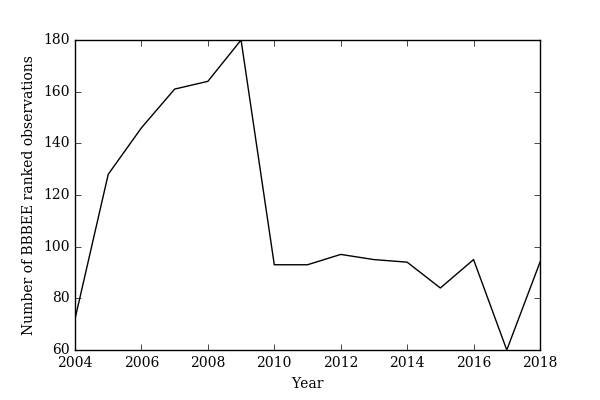
\includegraphics [scale=0.5]{ScatterPlot_Year_BBBEE_Rank.png} \\
  {\small {\it \caption{Available B-BBEE rank observations per year\label{fig:moun}}}}
\end{figure}
The B-BBEE ranks were retrieved through the Empowerdex top 100 JSE Most Empowered Companies, as mentioned in the methodology. Interestingly, it appears that the Empowerdex top 100 in pre 2010 mostly exceeded 100 firms. From 2010 onwards, the number of observations with a B-BBEE rank dropped to below 100 firms. The reason why the B-BBEE rank dropped below 100 firm, instead of equal to 100 firm as one would expect from a top 100, is that firms for which no price was available (price was retrieved from Thomson Reuters Datastream) were excluded. This resulted in an average of 5 firms being excluded, therefore an average of 95 firms available each year. Notably, in 2017 the number of firms dropped to 62. The B-BBEE rank for 2017 were retrieved from the Intellidex website. It appears that the amended codes were made obligatory by 2017, yielding in the drop of observations in 2017. The variability of observations required adjustments to prevent outcomes biased to the pre 2010 period. Put straightforward, as most observations were from pre 2010 this analysis would be moreso a reflection of the pre 2010 period, rather than the entire 2004 - 2018 period. Therefore, the number of B-BBEE rank was capped at 60, to create a uniform distribution of observations through time. In the use of the models, the B-BBEE rank was flipped, therefore rank 60 was the best ranking firm in terms of compliance to B-BBEE policy. This was done to improve readability of the regression results. In this case a negative coefficient for B-BBEE on share price returns indicates that the better the B-BBEE policy compliance of a firm, the worse the share price return.
\subsection{Control variables}
The risk free rate is defined as the yield on the 10 years South African Government bond. The yields of the 10 years South African Government bond is obtained through Thomson Reuters Datastream. The value factor is the book value per share as stated in Thomson Reuters Datastream. The book value per share equals the book market to market capitalization ratio. The size factor is the market capitalization factor and obtained through Thomson Reuters Datastream. The earnings to price ratio equals the earnings yield, which is defined as the earnings divided by the closing price of a firm. This ratio is retrieved from Thomson Reuters Datastream.

The Fama and French model uses three indices; market risk premium, BP Index and SIZE index. The constituents of these indices at any point in time depend on the universe of firms at that particular time. The availability of these firms depends on the availability of B-BBEE rank. Put straightforward, the  market risk premium is calculated as the average return of the firms available each year. The firms available each year depends on the availability of B-BBEE rank. The BP Index follows the Fama and French methodology, therefore the return of the BP Index equals the average return of the 30\% highest book to market ratio firms at a particular time minus the average return of the 30\% lowest book to market ratio firms at a particular time. The number of firms in total available, to emphasize, depends on the availability of B-BBEE rank. At the different time frames (one, two, three, four, five years) these indices represent the return of these indices over the different time frames, therefore the BP Index on a two years time frame represents the average two year return of the 30\% highest book to market ratio firms at a particular time minus the average return of the 30\% lowest book to market ratio firms at a particular time.

Instead of using industry categorization through the Code of Good Practise, this study based sector classification based on the ICB Industry name, which is gathered through the Thomson Reuters Datastream Industry Level 2 Sector Name. Using the sector classification from Thomson Reuters Datastream prevents the sector classification inconsistencies encountered in the Mokgobinyane study.

    
% Data
    %\chapter{Data}
    %\textcolor{red}{This Chapter should demonstrate that you have conducted a thorough and critical investigation of relevant sources.
Apart from a presentation of the sources of your data, this chapter allows you to critically discuss the data (whatever these data are, ‘quantitative’ or ‘qualitative’, primary or secondary), which is proof of good research. You can even do good research with poor data but you must demonstrate that you are aware of the data quality and accordingly are careful in your interpretations. Essentially, there are three aspects to consider:
\begin{enumerate}
\item	Reliability, which, for example, could depend on whether they are estimates or more direct evidence;
\item	Representativity, which is about how typical the data are; for example, you may have arguments why the very few cases are typical or you may carry out statistical tests;
\item Validity, which is about the relevance of the data for your case. Strictly speaking, sometimes no valid data are available but one may argue that there are other data which could be used as ‘proxies’.) 
\end{enumerate}
}
\section{Source Material}
Lorem ipsum dolor sit amet, consectetur adipiscing elit. Duis ut ipsum nec orci interdum sollicitudin ut eu nunc. Pellentesque ultricies eros in justo sagittis, eget blandit velit aliquet. Aenean ac lectus nibh. Quisque ac est pellentesque, ullamcorper sem sit amet, pharetra quam. Morbi ullamcorper placerat diam, sed tincidunt odio.


    
% Methods
    %\chapter{Methods}
    %\textcolor{red}{In this Chapter, you present in more concrete terms the method(s) you are going to apply. And as always in research, it is good to demonstrate awareness of the weaknesses or limitations of the method you use. It makes no difference if you work with interviews, econometric models, or a comprehensive analysis of data from various sources. Transparency should be the guideline: make it possible for your readers to follow, or even repeat, your analysis!}

\section{The Approach [or Model]}
Lorem ipsum dolor sit amet, consectetur adipiscing elit. Duis ut ipsum nec orci interdum sollicitudin ut eu nunc. Pellentesque ultricies eros in justo sagittis, eget blandit velit aliquet. Aenean ac lectus nibh. Quisque ac est pellentesque, ullamcorper sem sit amet, pharetra quam. Morbi ullamcorper placerat diam, sed tincidunt odio.
    
% Empirical Analysis
    \chapter{Empirical Analysis}
    This chapter discusses tests the hypothesis stated in the Methodology chapter. To arrive at the hypothesis tests, this chapter will first discuss the descriptives of the dataset used for analysis (hereafter, the analysis dataset). Thereafter the research sub questions are investigated.
\section{Descriptive statistics}
Descriptive statistics are used to inform the reader about the general characteristics of the analysis dataset used to test the hypotheses. Preferably these characteristics resemble the characteristics of the wider population to allow for generalized statements. Therefore, the firms from analysis dataset were compared to the JSE All Share Index. The JSE All Share Index is the broad based Index of the Johannesburg Stock Exchange. The table below compares the sector weighting for the B-BBEE sample and the JSE All Share Index (equal weighted) as of latest date. The equal weight of latest date for the JSE All Share Index was retrieved from Thomson Reuters Datastream. This index comprised as of latest date because only the latest date (as of 30th April 2019) and names (no weight) were available for the constituents of the JSE All Share Index. The sector weighting for the B-BBEE sample was calculated by the following formula:
\begin{equation}
\begin{aligned}
W_{it} = \frac{N_{it}}{N_{t}}
\end{aligned}
\end{equation}
where, $W_{it}$ is the sector weight of sector $i$ at time $t$, $N_{it}$ is the number of firm in sector $i$ at time $t$ and $N_{t}$ is the total number of firms at time $t$. 

For the JSE All Share the time variable was fixed, as only the latest date was available. To check for bias in the B-BBEE sample, this study subtracted the weight per sector of  JSE All Share Index from the analysis dataset per sector per time. Below the results.
\begin{table}[H] %H forces the position of the table at the line where you place it (not on a separate page etc) -https://tex.stackexchange.com/questions/121155/how-to-adjust-a-table-to-fit-on-page https://tex.stackexchange.com/questions/332528/increasing-the-space-between-two-rows?rq=1
\centering
\caption{Relative bias sample versus JSE All Share Index 2019} 
\resizebox{\textwidth}{!}{\begin{tabular}{ccccccccc}

  \bottomrule
  \\
 Year & Basic Materials & Consumer Goods & Consumer Services & Financials   & Healthcare   & Industrials & Technology   & Telecommunications \\ \\
  \midrule
2004 & 6\%             & 0\%            & 5\%               & -18\%      & -3\%       & 4\%         & 4\%        & 1\%                \\
2005 & 2\%             & 2\%            & -2\%              & -14\%      & -1\%       & 4\%         & 8\%        & 1\%                \\
2006 & 2\%             & 4\%            & 1\%               & -18\%      & -1\%       & 1\%         & 9\%        & 1\%                \\
2007 & 4\%             & -3\%           & 1\%               & -9\%       & -1\%       & -2\%        & 9\%        & 1\%                \\
2008 & -3\%            & -5\%           & -5\%              & -11\%      & -1\%       & 9\%         & 13\%       & 3\%                \\
2009 & -8\%            & -1\%           & 1\%               & -11\%      & 1\%        & 11\%        & 9\%        & -2\%               \\
2010 & -8\%            & -3\%           & -2\%              & -14\%      & 1\%        & 14\%        & 9\%        & 3\%                \\
2011 & -6\%            & -3\%           & -5\%              & -13\%      & 1\%        & 16\%        & 8\%        & 3\%                \\
2012 & -4\%            & -5\%           & -4\%              & -13\%      & -1\%       & 16\%        & 9\%        & 1\%                \\
2013 & -6\%            & -3\%           & -4\%              & -11\%      & 1\%        & 11\%        & 8\%        & 4\%                \\
2014 & -8\%            & -1\%           & -5\%              & -13\%      & 1\%        & 14\%        & 8\%        & 4\%                \\
2015 & -9\%            & -3\%           & -4\%              & -8\%       & 1\%        & 16\%        & 8\%        & -1\%               \\
2016 & -3\%            & -5\%           & -10\%             & -9\%       & -4\%       & 23\%        & 8\%        & 1\%                \\
2017 & -3\%            & -6\%           & 13\%              & -31\%      & 2\%        & 26\%        & -1\%       & -1\%               \\
2018 & -3\%            & -5\%           & -4\%              & -14\%      & -1\%       & 19\%        & 8\%        & -1\%  \\ 
   \bottomrule
\end{tabular}}
\end{table} 
This table shows the percentage of observations in any of the respective sectors for the JSE All Share equal weight, and the firms for which B-BBEE rank was available. Recall that the JSE All Share equal weight was retrieved from one point in time, therefore the percentage of observations in any of the sectors of the JSE All Share equal weight was static through time. The constituents, and therefore the weight of each sector for analysis dataset used however did change annually.

Comparing the analysis dataset with the JSE All Share indicate bias towards Industrials. This might be due to the nature of this sector and relates to the cross sectional dynamics of the relationship between B-BBEE policy and firm performance as found in the theoretical framework. Most firms in the Industrial sector were active in the construction business. In the construction business, it is likely that a significant portion either directly or indirectly engages in business with government entities. Recall from the Theory chapter, that firms that reach B-BBEE targets receive B-BBEE aggregate score that places these firms eligible to obtain government business and/or business from firms that require suppliers to be B-BBEE compliant  (\citeauthor{N7}, \citeyear{N7}, p546; \citeauthor{N3}, \citeyear{N3}; \citeauthor{N5}, \citeyear{N5}, p9). The extraordinary benefit Industrials enjoy, especially compared to other sectors, could explain the bias of the Industrial sector in the analysis dataset. It is interesting to note the increase in bias toward the Industrial sector in this dataset compared to the JSE All Share equal weight adjustment of the B-BBEE policy. This relates to the time dynamics as found in the theoretical framework. Recall from the Contextualization chapter that amendments in B-BBEE policy occurred in 2007 and in 2013. Prior to 2007 the overrepresentation of Industrials was about 4\%, between 2007 and 2013 about 15\%, and after 2013 24\%.

Contrary, the analysis dataset underrepresented the Financials sector. This also could be explained from the cross-sectional dynamic standpoint. Financials, such as banks, could have a less obvious benefits of B-BBEE compliance as these firms are not directly tendering on government like Industrial firms. However, recall from the Theory that consumer behavior could reward firms that were exhibiting social responsible behaviour \cite[p378]{N34}. This is benefit is however not found significant enough in the case of the Financials sector in the analysis dataset. The underrepresentation is somewhat surprising as the Contextualization chapter revealed Sanlam, a Financials sector firm, was the first South African firm to implement a form of BEE by transferring 10\% of ownership to Black people. The underrepresentation leads speculation that firms operating in the Financial sector mostly engage in B-BBEE policy to minimize damage and therefore adopt a defensive and apprehensive strategy reflected in the underrepresentation of this sector in the analysis dataset.

Despite these difference, the top 3 dominant sectors of the JSE All Share equal weight; Basic Materials, Consumer Service and Financials are also dominant in the analysis dataset. The smaller sectors; Technology, Health Care and Telecommunication displayed at most overseeable deviations between the analysis dataset and JSE All Share Index. The JSE All Share Index consisted of 164 firms, of which 125 were included in the analysis dataset at some point in time. Therefore, the analysis dataset was found representative of Johannesburg Stock Exchange listed firms.

The maximum amount of observations, given 60 firms for 15 years equals 900. Below an overview of descriptive statistics for the variables for Model 1, the FF (Fama and French based) model using the analysis dataset.  
\begin{table}[H] %H forces the position of the table at the line where you place it (not on a separate page etc) -https://tex.stackexchange.com/questions/121155/how-to-adjust-a-table-to-fit-on-page https://tex.stackexchange.com/questions/332528/increasing-the-space-between-two-rows?rq=1
\centering
\caption{Descriptive statistics variables} 
\resizebox{\textwidth}{!}{\begin{tabular}{ccccccccc}

  \bottomrule
  \\
 & BMRatio    & SIZERatio  & EPRatio  & BPIndex\_YR1 & SIZEIndex\_YR1 & MarketPremium\_YR1 & RiskFreeReturn\_YR1 & SharePriceReturn\_YR1 \\ \\
  \midrule
count & 816   & 900     & 835      & 15           & 15             & 15                 & 15                  & 900                 \\
mean  & 0.90  & 36024   & -11.50   & 6\%          & 2\%            & 9\%                & 8\%                 & 14\%                \\
std   & 2.42  & 96943   & 221.03   & 6\%          & 7\%            & 23\%               & 1\%                 & 47\%                \\
min   & -0.47 & 3       & -4670.81 & 0\%          & -15\%          & -20\%              & 7\%                 & -95\%               \\
25\%  & 0.34  & 1522    & 5.10     & 3\%          & -1\%           & -5\%               & 8\%                 & -12\%               \\
50\%  & 0.55  & 7653    & 7.70     & 6\%          & 4\%            & 3\%                & 9\%                 & 10\%                \\
75\%  & 0.88  & 26091   & 10.30    & 8\%          & 8\%            & 18\%               & 9\%                 & 31\%                \\
max   & 55.66 & 1434027 & 65.39    & 23\%         & 12\%           & 67\%               & 10\%                & 756\%     \\ 
   \bottomrule
\end{tabular}}
\end{table} 
The one year forward share price return varied widely. The standard deviation was 47.6\%, and the difference between the minimum and maximum observation share price return for one year equaled more than 800\%. Similarly the BM ratio and SIZE ratio varied greatly. BM is the book to market ratio as defined by Merwe and Ferreira. The minimum BM ratio was negative, indicating a firm with negative book value. This indicates negative equity value, or a company in severe distress. The number of observations on the BM ratio equaled 816, indicating that of 900 observations there was no BM ratio available for 84 observations. SIZE ratio was the market capitalization as defined by Merwe and Ferreira. The SIZE ratio indicates that both very small firms and very large firms were available in the dataset used for analysis. The indices, BM, SIZE, MarketPremium, and RiskFreeReturn only showed 1 value for each year, hence 15 observations were yielded for these variables. The indices of BP, SIZE, MarketPremium and RiskFreeReturn are based upon the Fama and French methodology. Recall that the RiskFreeReturn equals 10 years South African government bond. The RiskFreeReturn remained, compared to the other variables,  relatively immune from variability. The bottom 25 percentile  observation equaled 8.1\% and the top 75 percentile observation equaled 8.7\%.

Given the large variability of some of the factors, this study adjusted analysis dataset for outliers (hereafter, outlier adjusted analysis dataset). The outlier adjusted analysis dataset constrained the minimum value for the BM ratio, SIZE ratio, EP ratio and share price return to -2 times standard deviation from the mean, and the maximum value to +2 times standard deviation from the mean. The descriptives for this outlier adjusted analysis dataset are presented below.
\begin{table}[H] 
\centering
\caption{Descriptive statistics variables outlier adjusted} 
\resizebox{\textwidth}{!}{\begin{tabular}{ccccccccc}
  \bottomrule
  \\
 & BMRatio    & SIZERatio   & EPRatio      & BPIndex\_YR1 & SIZEIndex\_YR1 & MarketPremium\_YR1 & RiskFreeReturn\_YR1 & SharePriceReturn\_YR1 \\ \\
  \midrule
count & 816   & 900    & 835      & 15           & 15             & 14                 & 14                  & 900                 \\
mean  & 0.77  & 29618  & -11.50   & 4\%          & 4\%            & 4\%                & 17\%                & 14\%                \\
std   & 0.79  & 52727  & 221.03   & 3\%          & 4\%            & 21\%               & 1\%                 & 40\%                \\
min   & -0.47 & 3      & -4670.81 & 0\%          & -3\%           & -27\%              & 15\%                & -95\%               \\
25\%  & 0.34  & 1522   & 5.10     & 2\%          & 1\%            & -7\%               & 17\%                & -12\%               \\
50\%  & 0.55  & 7653   & 7.70     & 4\%          & 3\%            & 1\%                & 18\%                & 10\%                \\
75\%  & 0.88  & 26091  & 10.30    & 6\%          & 6\%            & 7\%                & 18\%                & 31\%                \\
max   & 4.84  & 225857 & 65.39    & 11\%         & 12\%           & 50\%               & 19\%                & 189\%      \\
   \bottomrule
\end{tabular}}
\end{table} 
Recall that the indices of BM, SIZE and MarketPremium were based on the universe of share price returns available. Therefore, adjusting the share price return for outliers also impacted the indices of BM, SIZE and MarketPremium. The outlier adjusted analysis dataset still displayed variability, however at a much lower rate as can be viewed from the significantly lower maximum value for BMRatio, SIZERatio and share price return. It is interesting to note that the variability of the MarketPremium rose as result of the outlier adjustment for the share price return. This indicates that as outliers were excluded from share price return, correlations increased between firms share price return and therefore the variability of the MarketPremium increased.

The correlation matrix suggests that multicollinearity did not exist in the analysis dataset. Below the correlation matrix for the analysis dataset.
\begin{table}[H] 
\centering
\caption{Correlation matrix} 
\resizebox{\textwidth}{!}{\begin{tabular}{rrrrrrrrrr}
  \bottomrule
     & 1     & 2     & 3     & 4     & 5     & 6     & 7     & 8     & 9 \\
  \midrule
BMRatio (1)                  & 1.00  & -0.08 & -0.02 & 0.01  & -0.04 & -0.07 & 0.04  & 0.04  & -0.05 \\
SIZERatio (2)                & -0.08 & 1.00  & 0.03  & -0.03 & -0.05 & 0.06  & -0.04 & -0.06 & 0.04  \\
EPRatio (3)                 & -0.02 & 0.03  & 1.00  & 0.03  & -0.02 & 0.01  & 0.05  & 0.00  & 0.08  \\
BPIndex\_YR1 (4)        & 0.01  & -0.03 & 0.03  & 1.00  & 0.00  & -0.11 & -0.34 & 0.06  & -0.20 \\
BBBEE\_Rank (5)         & -0.04 & -0.05 & -0.02 & 0.00  & 1.00  & 0.00  & 0.00  & 0.00  & -0.03 \\
SIZEIndex\_YR1 (6)      & -0.07 & 0.06  & 0.01  & -0.11 & 0.00  & 1.00  & -0.60 & -0.28 & -0.15 \\
MarketPremium\_YR1 (7)  & 0.04  & -0.04 & 0.05  & -0.34 & 0.00  & -0.60 & 1.00  & -0.07 & 0.39  \\
RiskFreeReturn\_YR1 (8) & 0.04  & -0.06 & 0.00  & 0.06  & 0.00  & -0.28 & -0.07 & 1.00  & -0.05 \\
SharePriceReturn\_YR1 (9) & -0.05 & 0.04  & 0.08  & -0.20 & -0.03 & -0.15 & 0.39  & -0.05 & 1.00                 \\ 
   \bottomrule
\end{tabular}}
\end{table} 
An overview of the correlations on two, three, four and five years basis can be found in Appendix A. The correlation matrix for the outlier adjusted analysis dataset shows as similar picture, as can be viewed below.
\begin{table}[H] 
\centering
\caption{Correlation matrix} 
\resizebox{\textwidth}{!}{\begin{tabular}{rrrrrrrrrr}
  \bottomrule
     & 1     & 2     & 3     & 4     & 5     & 6     & 7     & 8     & 9 \\
  \midrule
BMRatio (1)                  & 1.00  & -0.23 & -0.08 & 0.02  & -0.02 & 0.03  & -0.10 & 0.06  & -0.17 \\
SIZERatio (2)                & -0.23 & 1.00  & 0.04  & 0.00  & -0.03 & 0.04  & -0.01 & -0.08 & 0.06  \\
EPRatio (3)                 & -0.08 & 0.04  & 1.00  & 0.05  & -0.02 & 0.04  & 0.05  & 0.00  & 0.09  \\
BPIndex\_YR1 (4)        & 0.02  & 0.00  & 0.05  & 1.00  & 0.00  & 0.53  & -0.34 & -0.12 & -0.16 \\
BBBEE\_Rank (5)         & -0.02 & -0.03 & -0.02 & 0.00  & 1.00  & 0.00  & 0.00  & 0.00  & -0.01 \\
SIZEIndex\_YR1 (6)      & 0.03  & 0.04  & 0.04  & 0.53  & 0.00  & 1.00  & -0.65 & -0.29 & -0.24 \\
MarketPremium\_YR1 (7)  & -0.10 & -0.01 & 0.05  & -0.34 & 0.00  & -0.65 & 1.00  & -0.27 & 0.46  \\
RiskFreeReturn\_YR1 (8) & 0.06  & -0.08 & 0.00  & -0.12 & 0.00  & -0.29 & -0.27 & 1.00  & -0.05 \\
SharePriceReturn\_YR1 (9) & -0.17 & 0.06  & 0.09  & -0.16 & -0.01 & -0.24 & 0.46  & -0.05 & 1.00                \\ 
   \bottomrule
\end{tabular}}
\end{table} 
Both correlation matrices indicate that there is no multicollinearity within the datasets. The observed correlations between the variables are low to negative. The correlation matrix for the outlier adjusted analysis dataset shows more pronounced correlations as expected. For example the correlation between BM ratio and SIZE ratio is -0.23 in the outlier adjusted analysis dataset versus -0.08 in the analysis dataset.

It can also be observed from the correlation matrix of the analysis dataset that the market, contrary intuition based on the Fama French theory, indicates a negative correlations between BM ratio and share price return and BM Index and share price return. Recall from the Theory chapter that Fama and French state that the market undervalues distressed, high book to market ratio firms, and therefore these firms tend to outperform low book to market ratio firms \cite[p1975]{N52}. This relationship is elusive in the analysis dataset. This indicates that this variable could be inappropriate to explain share price returns within the analysis dataset. On the other hand the correlation between MarketPremium and  share price return did display a higher correlation, 0.46. Therefore, the analysis dataset suggests that share price return for firms was mostly determined by movement of the general market. This, in the context of a developing/emerging market such as South Africa, seems perfectly logical as these markets are not as mature as the United States, Japanese or European markets upon which the Fama French study were based. Nonetheless the unexpected correlation between BM and share price return does raise concerns on the appropriateness of BM as a control variable in this study.
\section{Regression results}
Recall that the methodology indicated three aspects to the relationship between B-BBEE policy and firm performance, one calling for analysis the entire dataset, one calling for regression of specific time periods and one calling for regressions per sector. This section presents the empirical results of the regression analysis per sub research question by operationalizing B-BBEE policy through B-BBEE rank and firm performance with share price return, per specification in the Methodology chapter.
\subsection{Relationship between B-BBEE policy and firm performance 2004 -2018}
This section concerns the research sub question: “What was the long term relationship between  Broad-Based Black Economic Empowerment policy on firm performance of the Johannesburg Stock Exchange-listed companies over the period 2004 - 2018?”. The regression results of  analysis dataset for this sub research question for Model 1, the FF model (specified in the Methodology chapter) looks as follows:
\begin{table}[H] 
\tiny %https://tex.stackexchange.com/questions/27097/changing-the-font-size-in-a-table
\centering
\caption{Regression Model 1, 2004 - 2018} 
\resizebox{\textwidth}{!}{\begin{tabular}{lrrrrr}
  \bottomrule
     &     1     &     2     &     3      &     4     &     5      \\
  \midrule
BMIndex                 & -0.2480   & -0.4555   & -1.1840    & 0.3650    & 1.2904     \\
                   & (0.3197)  & (0.8511)  & (1.5824)   & (2.5089)  & (2.1644)   \\
BBBEE\_Rank         & -0.0006   & -0.0028*  & -0.0069*** & -0.0065*  & -0.0017    \\
                   & (0.0009)  & (0.0016)  & (0.0026)   & (0.0034)  & (0.0046)   \\
SIZEIndex               & 0.8076**  & 0.5197    & 0.6443     & 0.6603    & -0.1533    \\
                   & (0.3248)  & (0.5360)  & (0.7693)   & (1.1358)  & (1.1300)   \\
MarketPremium      & 0.9686*** & 1.0702*** & 1.1230***  & 1.4520*** & 1.6534***  \\
                   & (0.1079)  & (0.1748)  & (0.3680)   & (0.5178)  & (0.3945)   \\
RiskFreeReturn     & 0.6521    & -0.1951   & 0.8228     & -2.7341   & -4.1080    \\
                   & (2.2691)  & (2.9432)  & (3.6206)   & (7.5388)  & (7.9526)   \\
Consumer Goods     & 0.0369    & 0.2265    & 0.1400     & 1.7100    & 2.9063     \\
                   & (0.2143)  & (0.5548)  & (1.0675)   & (2.9893)  & (4.0711)   \\
Financials         & 0.0558    & 0.3282    & 0.3099     & 1.8070    & 2.9933     \\
                   & (0.2090)  & (0.5489)  & (1.0607)   & (2.9764)  & (4.0449)   \\
Technology         & -0.0488   & 0.2580    & 0.2805     & 1.8074    & 3.0038     \\
                   & (0.2127)  & (0.5551)  & (1.0666)   & (2.9762)  & (4.0513)   \\
Healthcare         & 0.0960    & 0.5821    & 0.5522     & 2.1466    & 3.4400     \\
                   & (0.2165)  & (0.5585)  & (1.0739)   & (2.9911)  & (4.0623)   \\
Industrials        & -0.0384   & 0.1635    & 0.0480     & 1.4233    & 2.2926     \\
                   & (0.2061)  & (0.5464)  & (1.0565)   & (2.9752)  & (4.0371)   \\
Consumer Services  & 0.0634    & 0.2392    & 0.1807     & 1.6321    & 2.7102     \\
                   & (0.2102)  & (0.5533)  & (1.0664)   & (2.9819)  & (4.0610)   \\
Basic Materials    & 0.0184    & 0.1657    & 0.0090     & 1.5287    & 2.4668     \\
                   & (0.2115)  & (0.5537)  & (1.0651)   & (2.9778)  & (4.0566)   \\
Telecommunications & 0.0742    & 0.2379    & 0.1742     & 1.5765    & 2.4642     \\
                   & (0.2201)  & (0.5583)  & (1.0682)   & (2.9831)  & (4.0483)   \\
N                  & 816       & 752       & 694        & 638       & 582        \\
R^2                 & 0.18      & 0.22      & 0.26       & 0.14      & 0.10       \\
   \bottomrule
Standard errors in parentheses.
* p<0.10, ** p<0.05, ***p0.01\
\end{tabular}}
\end{table} 
There are 5 columns visible in this table, these tables represent the share price returns time horizon. Therefore column 1 represent the 1 year share price return, column 2 represents the two year forward share price return, etc. From this model, under the specifications stated (no adjustment for outliers), r-squared for all time horizons exceed 0.10. Merwe and Ferreira (\citeyear{N7}, p551), in their study, note that a r-squared of 5.6\% is acceptable to investigate the relationship between B-BBEE score and share price return. Therefore, Model 1’s r-squared of equal to or exceeding 0.10, is interpreted as sufficient to capture the relationship between B-BBEE rank and share price return. 

Model 1 finds negative relationships between B-BBEE rank and share price return, significant on a two, three and four years time horizon. This means that for the specified time horizons, the better the B-BBEE rank, the worse the share price return. It has to be noted that the magnitude, especially compared to the coefficients of other independent variables is small. For example, the three year regression shows the most negative B-BBEE rank coefficient of -0.0069. This indicates that an 1 incremental improvement of B-BBEE rank results in a reduction on a two years share price return of merely 0.69\%. Recall from the descriptives section that the variability of share price return was quite high (non outlier adjusted standard deviation of 47\%), therefore the impact that a change in B-BBEE rank has on two years share price return is quite muted.  In comparison, the magnitude of the market premium is far larger, and significant over the five time horizons. This suggests that the impact of B-BBEE is relatively small, but negative. Merwe and Ferreira (\citeyear{N7}, p552) also observed a same small significant negative relationship between B-BBEE and share price return. Using the different time horizons, Model 1 adds to the finding of Merwe and Ferreira and shows that the negative coefficient of B-BBEE rank increases up until the 4 years time horizon, from -0.0006 to -0.065. The increase of magnitude follows suggestions by Mehta and Ward (\citeyear{N27}, p89) who indicated that the market has an initial response to a B-BBEE rank, which is more positive, and as the market processes information, the response to the B-BBEE rank becomes more pronounced. The negative increasing coefficient and significance of the relationship between B-BBEE rank and share price performance over various share price return time horizons indicate that the costs of B-BBEE policy compliance for firm outweigh the benefits, causing a negative long term relationship between B-BBEE policy and firm performance.

To check for robustness, the same model was tested on the outlier adjusted analysis dataset. Below the results.
\begin{table}[H] 
\tiny %https://tex.stackexchange.com/questions/27097/changing-the-font-size-in-a-table
\centering
\caption{Regression Model 1 - outlier adjusted, 2004 - 2018} 
\resizebox{\textwidth}{!}{\begin{tabular}{lrrrrr}
  \bottomrule
     &     1     &     2     &     3      &     4     &     5      \\
  \midrule
BMIndex                 & -0.4858   & -1.8037   & -2.0434   & -2.5375*  & -1.0682   \\
                   & (0.4961)  & (1.2019)  & (1.5805)  & (1.4165)  & (1.7208)  \\
BBBEE\_Rank         & 0.0002    & -0.0023*  & -0.0040** & -0.0046** & -0.0031   \\
                   & (0.0008)  & (0.0012)  & (0.0018)  & (0.0023)  & (0.0031)  \\
SIZEIndex               & 1.4892*** & 1.4440*** & 1.9992*** & 1.5684*   & 0.7834    \\
                   & (0.5035)  & (0.4597)  & (0.5777)  & (0.8307)  & (1.2044)  \\
MarketPremium      & 0.9909*** & 0.7264*** & 0.5739    & 0.6428    & 0.9448**  \\
                   & (0.0889)  & (0.2324)  & (0.4437)  & (0.3912)  & (0.3946)  \\
RiskFreeReturn     & -0.9639   & -5.2936** & -6.9621** & -3.7378   & -4.6235   \\
                   & (2.3277)  & (2.4482)  & (3.0451)  & (2.5987)  & (3.0165)  \\
Consumer Goods     & 0.1620    & 1.1208*** & 2.2522*** & 2.0092**  & 3.1361**  \\
                   & (0.2098)  & (0.4083)  & (0.7774)  & (0.9581)  & (1.4945)  \\
Financials         & 0.1339    & 1.1070*** & 2.1980*** & 1.9381**  & 3.0821**  \\
                   & (0.2058)  & (0.4012)  & (0.7659)  & (0.9435)  & (1.4760)  \\
Technology         & 0.0557    & 1.0409**  & 2.0749*** & 1.5954*   & 2.5532*   \\
                   & (0.2091)  & (0.4069)  & (0.7730)  & (0.9501)  & (1.4821)  \\
Healthcare         & 0.2218    & 1.3349*** & 2.5125*** & 2.3881**  & 3.7449**  \\
                   & (0.2115)  & (0.4115)  & (0.7734)  & (0.9552)  & (1.4895)  \\
Industrials        & 0.0540    & 0.9886**  & 1.9611**  & 1.5478*   & 2.4982*   \\
                   & (0.2035)  & (0.3977)  & (0.7609)  & (0.9391)  & (1.4675)  \\
Consumer Services  & 0.1520    & 1.1381*** & 2.2232*** & 1.8841**  & 2.9608**  \\
                   & (0.2070)  & (0.4056)  & (0.7723)  & (0.9489)  & (1.4848)  \\
Basic Materials    & 0.1664    & 1.0613*** & 2.1641*** & 1.7577*   & 2.7730*   \\
                   & (0.2072)  & (0.4061)  & (0.7780)  & (0.9528)  & (1.4871)  \\
Telecommunications & 0.1557    & 1.1154*** & 2.2015*** & 1.7467*   & 2.6537*   \\
                   & (0.2129)  & (0.4132)  & (0.7783)  & (0.9564)  & (1.4832)  \\
N                  & 757       & 693       & 635       & 579       & 523       \\
R^2                 & 0.24      & 0.20      & 0.14      & 0.15      & 0.14      \\
   \bottomrule
Standard errors in parentheses.
* p<0.10, ** p<0.05, ***p<0.01
\end{tabular}}
\end{table} 
Here the relationship between B-BBEE rank and share price return on a one-year time horizon is slightly positive albeit not significant. On the two, three and four years time horizon, the relationship between B-BBEE rank and share price returns remains, just as in the analysis dataset,  negative and significant, but at slightly less negative coefficient compared to the analysis dataset. In contrast the 5 years time horizon displays a more pronounced negative coefficient, compared to the non outlier adjusted model. Therefore, the outlier adjusted Model 1 suggest that outliers did indeed impact the analysis dataset. However, the finding from Model 1 for the analysis dataset, displaying significant negative relationships between B-BBEE rank and share price return on various time horizons remained intact.

Using the Model 2, based on the Merwe and Ferreira model the analysis dataset yields the following results:
\begin{table}[H] 
\tiny %https://tex.stackexchange.com/questions/27097/changing-the-font-size-in-a-table
\centering
\caption{Regression Model 2, 2004 - 2018} 
\resizebox{\textwidth}{!}{\begin{tabular}{lrrrrr}
  \bottomrule
     &     1     &     2     &     3      &     4     &     5      \\
  \midrule
const              & 0.1734*** & 0.3719*** & 0.6843*** & 0.8264*** & 0.8976***  \\
                   & (0.0343)  & (0.0633)  & (0.1052)  & (0.1258)  & (0.1680)   \\
BMRatio                 & -0.0078   & 0.0452*** & 0.0617*** & 0.0560**  & 0.0518*    \\
                   & (0.0071)  & (0.0125)  & (0.0201)  & (0.0232)  & (0.0296)   \\
SIZERatio               & 0.0000    & -0.0000   & -0.0000*  & -0.0000   & -0.0000    \\
                   & (0.0000)  & (0.0000)  & (0.0000)  & (0.0000)  & (0.0000)   \\
EPRatio                & 0.0001*   & 0.0006*** & 0.0006*   & 0.0007*   & 0.0027*    \\
                   & (0.0001)  & (0.0002)  & (0.0003)  & (0.0004)  & (0.0014)   \\
BBBEE\_Rank         & -0.0004   & -0.0024   & -0.0065** & -0.0068*  & -0.0016    \\
                   & (0.0010)  & (0.0018)  & (0.0030)  & (0.0036)  & (0.0048)   \\
Consumer Goods     & 0.0562    & 0.1012    & 0.1306    & 0.1914    & 0.2939     \\
                   & (0.0573)  & (0.1038)  & (0.1694)  & (0.2020)  & (0.2689)   \\
Financials         & 0.0388    & 0.0791    & 0.1678    & 0.2121    & 0.2970*    \\
                   & (0.0363)  & (0.0653)  & (0.1084)  & (0.1305)  & (0.1744)   \\
Technology         & -0.0606   & -0.0277   & 0.0457    & 0.1290    & 0.3067     \\
                   & (0.0525)  & (0.0934)  & (0.1542)  & (0.1832)  & (0.2435)   \\
Healthcare         & 0.0550    & 0.3260**  & 0.3339    & 0.4978*   & 0.7604**   \\
                   & (0.0761)  & (0.1421)  & (0.2277)  & (0.2754)  & (0.3714)   \\
Industrials        & -0.0838** & -0.1404** & -0.1430   & -0.1942   & -0.3659**  \\
                   & (0.0363)  & (0.0674)  & (0.1136)  & (0.1371)  & (0.1833)   \\
Consumer Services  & 0.0507    & 0.0393    & 0.0932    & 0.0534    & 0.0341     \\
                   & (0.0441)  & (0.0839)  & (0.1367)  & (0.1621)  & (0.2140)   \\
Basic Materials    & 0.0523    & -0.0467   & -0.0752   & -0.1002   & -0.2772    \\
                   & (0.0456)  & (0.0834)  & (0.1389)  & (0.1633)  & (0.2147)   \\
Telecommunications & 0.0647    & 0.0411    & 0.1312    & 0.0371    & -0.1515    \\
                   & (0.0828)  & (0.1491)  & (0.2471)  & (0.2904)  & (0.3949)   \\
N                  & 816       & 752       & 694       & 638       & 582        \\
R^2                 & 0.02      & 0.04      & 0.04      & 0.03      & 0.04       \\
   \bottomrule
Standard errors in parentheses.
* p<0.10, ** p<0.05, ***p<0.01
\end{tabular}}
\end{table} 
It is immediately visible that the r-squared of Model 2 which follows the Merwe and Ferreira model lags the Model 1 which followed the Fama French model more closely. This strengthens the belief that the control variables as used in the Fama French model are more appropriate to explain share price return. Model 1 is significant on two, three and four years returns and Model 2  is significant on three and four years. Merwe and Ferreira (\citeyear{N7}, p552) use B-BBEE score rather than B-BBEE rank and found a coefficient of -0.003 at 1\% significant between B-BBEE score and share price return. The Merwe and Ferreira finding means that an one increment increase of B-BBEE score detracts 0.30\% of one year share price return. This coefficient differs from the finding presented in this study, when comparing this finding with the 1 year time horizon model as this study finds a (insignificant) coefficient nearly close to zero, -0.0004. This difference could arise from time period bias in the Merwe and Ferreira research as Merwe and Ferreira use the time period of 2005 - 2011, whereas this study analyzes the time period 2004 - 2018.

Nonetheless, the findings of Model 2 on the relationship between B-BBEE rank and share price return are largely unchanged. The coefficients for the relationship between B-BBEE rank and share price return at most differ -0.0004. This means that for the entire time period of 2004 to 2018 a higher B-BBEE rank did not add to share price returns.
\subsection{Relationship between B-BBEE policy on firm performance in three B-BBEE policy periods}
This section deals with the research sub question: “What was the relationship between B-BBEE policy and firm performance among the three B-BBEE policy periods?”. Previous research on the relationship between B-BBEE and firm performance did not show consensus on the nature of the relationship. This could be due to the different time periods the studies used. It could be that the overall nature between B-BBEE and firm performance was negative, but that a particular time periods the relationship was positive. It could also be that the negative relationship over the entire dataset found in the previous section is driven by a particular time period. This study examined the relationship over the three periods of B-BBEE, as explained in the Methodology. The three sections this study identified where from 2004 until 2007, from 2007 until 2013 and from 2013 until 2018. These sections were selected based on B-BBEE policy initiation in 2004 and B-BBEE policy amendments in 2007 and 2013. Below the relationships between B-BBEE rank and share price returns over the three periods.

The period 2004 to 2007 shows the following regression results for the analysis dataset using Model 1:
\begin{table}[H] 
\tiny %https://tex.stackexchange.com/questions/27097/changing-the-font-size-in-a-table
\centering
\caption{Regression Model 1, sub sections} 
\resizebox{\textwidth}{!}{\begin{tabular}{lrrrrr}
  \bottomrule
     &     1     &     2     &     3      &     4     &     5      \\
  \midrule
BBBEE\_Rank 2004 - 2007        & -0.0036  & 0.0032   & -0.0066  & -0.0084  & -0.0028    \\
                   & (0.0032) & (0.0055) & (0.0081) & (0.0073) & (0.0067)   \\
BBBEE\_Rank 2007 - 2013        & 0.0009    & -0.0030  & -0.0054*  & -0.0033   & 0.0008     \\
                   & (0.0009)  & (0.0019) & (0.0032)  & (0.0050)  & (0.0070)   \\
BBBEE\_Rank 2013 - 2018       & -0.0002   & -0.0060*** & -0.0083*** & -0.0123*** & -0.0088    \\
                   & (0.0013)  & (0.0020)   & (0.0030)   & (0.0040)   & (0.0061)   \\                   
   \bottomrule
Standard errors in parentheses.
* p<0.10, ** p<0.05, ***p<0.01
\end{tabular}}
\end{table} 
The period 2004 - 2007 shows no significant relationship between between B-BBEE rank and share price return. Recall from the chronology discussed in earlier section that this was a period in which B-BBEE policy was not enforced tightly. The results over time do display that increasing interventionist stance of the B-BBEE became more pronounced in share price return. the relationship between B-BBEE rank and one and five year share price return were marginally positive. With regards to the 2007 to 2013 period, the relationship between B-BBEE and share price returns on two, three and four years basis were less negative compared to the entire dataset results. It has to be noted that these findings, with the exception of the three years regression, were not significant. These findings resemble the findings of Mokgobinyane who found a disperse relationship between the B-BBEE score coefficients on different measurements of firm performance using observations from this time period. Finally, with regards to the 2013 to 2018 period, it is found that this time period produces the most pronounced negative relationships between B-BBEE rank and share price return. The negative coefficients of B-BBEE rank on the two, three and four years share price return were found significant on 1\%. The descriptive statistics section of this chapter, this study observed that the bias toward Industrials, a sector more dependent on B-BBEE compliance, increased as the Codes of Practise became more stringent over time. However, this study finds that the benefits of B-BBEE compliance over the 2013 to 2018 did not outweigh the costs. This finding contrasts Acemoglu et al. (\citeyear{N23}, p32), who finds positive, but not significant, relationship between B-BBEE aggregate score and net profit margin. It could be however, especially consider the short time span, that a disconnect existed between net profit margins and share price returns. For example, Merwe and Ferreira (\citeyear{N7}, p552)  examined the period 2005 to 2011, which therefore overlaps the period 2004 to 2007 and found a small significant negative relationship between B-BBEE and share price return. The analysis of the different sub-sections of time indicate that increasing intervention of B-BBEE policy caused a more pronounced negative relationship between B-BBEE policy and share price return.
\subsection{Relationship between B-BBEE policy on firm performance on sector basis}
The theoretical framework also identified cross-sectional dynamics to hypothetically affect the relationship between B-BBEE policy. The theory notes that the aggregate cost and benefit for firms to comply to the B-BBEE policy might differ across sectors. This relates to the sub research question: “Did the relationship between B-BBEE policy and firm performance differ across sectors?”. Therefore the analysis dataset was subdivided per sector. The next table displays result of the sector linear regressions using Model 1 per sector.
\begin{table}[H] 
\tiny %https://tex.stackexchange.com/questions/27097/changing-the-font-size-in-a-table
\centering
\caption{Regression Model 1, sub sections} 
\resizebox{\textwidth}{!}{\begin{tabular}{lrrrrr}
  \bottomrule
     &     1     &     2     &     3      &     4     &     5      \\
  \midrule
BBBEE\_Rank\_Telecom      & -0.0012  & 0.0006     & -0.0005    & -0.0082    & -0.0221   \\
                          & -0.0041  & -0.0075    & -0.0107    & -0.0132    & -0.0191   \\
BBBEE\_Rank\_BasicMat     & 0.0007   & -0.0008    & -0.0045    & -0.011     & -0.009    \\
                          & -0.0031  & -0.0049    & -0.0067    & -0.0078    & -0.0083   \\
BBBEE\_Rank\_ConsumerServices & 0.0019   & -0.001     & -0.0042    & -0.0069    & -0.0094   \\
                          & -0.0014  & -0.0025    & -0.0036    & -0.0056    & -0.0067   \\
BBBEE\_Rank\_Industrials  & -0.0027* & -0.0125*** & -0.0182*** & -0.0201*** & -0.0132*  \\
                          & -0.0016  & -0.0027    & -0.0047    & -0.006     & -0.007    \\
BBBEE\_Rank\_HealthCare   & -0.0005  & 0.0069     & -0.0016    & 0.0052     & 0.0084    \\
                          & -0.0039  & -0.0095    & -0.0087    & -0.0098    & -0.0214   \\
BBBEE\_Rank\_Technology   & 0.0012   & -0.0042    & -0.0009    & 0.014      & 0.0365    \\
                          & -0.0033  & -0.0076    & -0.0141    & -0.0237    & -0.0363   \\
BBBEE\_Rank\_Financials   & -0.0019  & 0.0024     & 0.0012     & 0.0041     & 0.0071    \\
                          & -0.0022  & -0.0039    & -0.0064    & -0.0068    & -0.0091   \\
BBBEE\_Rank\_ConsumerGoods & 0.0011   & 0.0053**   & 0.0024     & 0.0032     & 0         \\
                          & -0.0019  & -0.0026    & -0.0038    & -0.0047    & -0.0068   \\
                          &          &            &            &            &           \\
N\_Telecom                & 32       & 30         & 28         & 27         & 23        \\
N\_BasicMat               & 117      & 101        & 93         & 89         & 84        \\
N\_ConsumerServices           & 124      & 100        & 97         & 90         & 84        \\
N\_Industrials            & 221      & 179        & 158        & 141        & 125       \\
N\_HealthCare             & 35       & 29         & 29         & 26         & 23        \\
N\_Technology             & 91       & 84         & 78         & 72         & 66        \\
N\_Financials             & 215      & 197        & 180        & 162        & 147       \\
N\_ConsumerGoods           & 215      & 197        & 180        & 162        & 147         \\                   
   \bottomrule
Standard errors in parentheses.
* p<0.10, ** p<0.05, ***p<0.01
\end{tabular}}
\end{table} 
The sectors Consumer Goods, Technology, Health Care and Telecom have less than 100 observations on one year time horizon. Considering 15 years, that means that these sector could exhibit time period bias. The Model 1 for these sectors are mostly insignificant with varying coefficients. Only the Consumer Goods sector on a two years horizon shows significant negative relationship between B-BBEE policy and firm performance. However, due to the insignificance of most relationships and the low observation count, it is difficult to state substantial claims based on these sectors.

The relationship between B-BBEE policy and firm performance for Financials is found insignificant but positive. This contradicts suspicions raised in the descriptive statistics section, where underrepresentation towards Financials hinted towards possible low benefits of B-BBEE compliance to Financials. This finding of insignificant but positive relationship between B-BBEE policy and firm performance for this sector could hint that firms that do decide to comply to B-BBEE policy find that benefits are greater than costs. This insignificant positive relationship demands further investigation.

Most interestingly, the sectors in which the incentives to comply, access to government contracts, was expected larger, display negative relationship between B-BBEE policy and firm performance. Most notable, the Industrial sector shows highly significant and most pronounced negative coefficients. This indicates that the benefits presented for these firm to comply to B-BBEE policy are underwhelming compared to the costs. It is further interesting to note that for Industrial to coefficient becomes more pronounced negative as time horizon increases, until the four year time horizon. This indicates that especially on the longer term the relationship between B-BBEE policy and firm performance is negative and favors the notion from the Theory that the incentive to comply to B-BBEE by providing access is, acts more as a cost to continue to do business. 
\section{Bootstrap method}
To add robustness to the findings from the regression analysis, this study investigated whether the relationship between B-BBEE rank and share price return displayed a deviating result using the Bootstrap method as stated by Mehta and Ward. This adds robustness to answer the research sub questions “What was the long term relationship between Broad-Based Black Economic Empowerment policy on firm performance of the Johannesburg Stock Exchange-listed companies over the period 2004 - 2018?” and  “Did the relationship between B-BBEE policy and firm performance differ across sectors?”. Below a visualization of the bootstrap method results.
\begin{figure}[H]
  \centering
  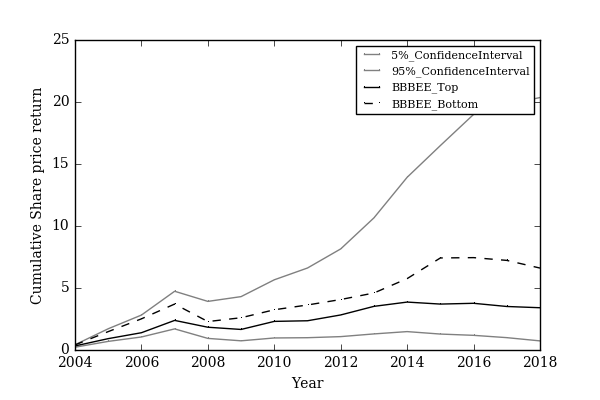
\includegraphics [scale=1]{Images/Bootstrap_All.png} \\
  {\small {\it \caption{Bootstrap entire dataset \label{fig:moun} }}}
\end{figure}
This chart displays four variables the 5\% and 95\% confidence intervals and the share price return of the top and bottom B-BBEE ranking firms. The confidence intervals were generated by bootstrapping the average returns of the entire dataset for each year, and retrieving the 5\% lowest and 5\% highest average returns for this year. These returns, as well as the returns for the top and bottom B-BBEE ranking firms were compounded over time. The top and bottom B-BBEE ranking firms were the average return of top and bottom 30\% ranking firms for each years. This chart shows that the 5\% highest average returns, the 95\% confidence interval rose significantly post 2008, outperforming all other variables handsomely as the average returns compounded aggressively. Similarly, although at a significant smaller compounding rate, the bottom B-BBEE ranking firms rose after 2008. It is particularly striking that from this analysis the bottom ranking B-BBEE firms outperform the top ranking B-BBEE firms. This analysis further shows the the bottom ranking B-BBEE firms do outperform the 5\% low confidence interval. This indicates the relationship between B-BBEE and share price return is insignificant, but most likely negative. Therefore this analysis provides (weak) support to the finding of the regression analyses on the entire period 2004 to 2018.

Returning towards a possible bias in the Industrial sector, this study performed the same bootstrap analysis for firms in this sector to answer the sub question: “Did firms operating in a sector with a higher incentive to comply to the B-BBEE policy have higher firm performance?” Below a visualization of the results. 
\begin{figure}[H]
  \centering
  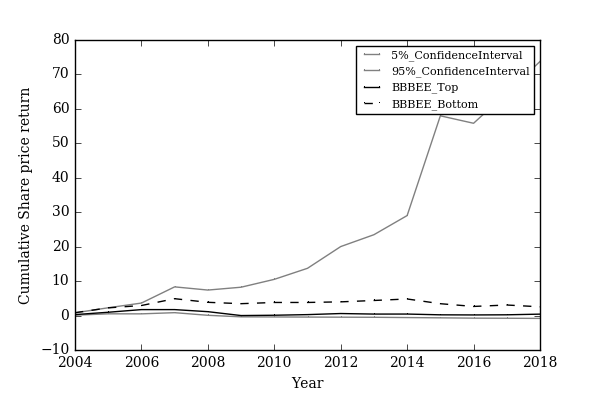
\includegraphics [scale=1]{Images/Bootstrap_Industrials.png} \\
  {\small {\it \caption{Bootstrap Industrials \label{fig:moun} }}}
\end{figure}
The above bootstrap analysis on the Industrial sector did entail a smaller sample size, which might explain that the findings of this chart are an exaggeration of the findings in the bootstrap analysis on the entire dataset. This chart, contrary to the idea in the Descriptives section, it appears that the negative relationship between B-BBEE and share price return is close to significant, as the top B-BBEE ranking firms in the Industrial sector remain close to the bottom 5\% confidence interval. This confirms earlier findings from the regression analysis on a sector by sector basis. 

The simulation for Consumer Services also shows a non significant performance of the top ranking B-BBEE firms. This can be seen below.
\begin{figure}[H]
  \centering
  \includegraphics [scale=1]{"Images/Bootstrap_Consumer Services_Cumulative"} \\
  {\small {\it \caption{Bootstrap Consumer Services \label{fig:moun} }}}
\end{figure}
This sector, however, does display that the top ranking B-BBEE firms outperformed the bottom ranking B-BBEE firms. Recall, from the Theory states that  consumer behavior could express their values regarding empowerment in their consumption pattern \cite[p378]{N34}. This chart shows weak evidence of this statement. This effect supports the Financial sector regression finding that firms with no direct or indirect government access could benefit from B-BBEE policy compliance.

The other sector bootstrap simulation can be found in Appendix C. Note however, that the sectors Telecommunications, Technology, Health Care and Consumer Goods had only a limited number of observations in each year. This could affect the robustness of the findings per sector. 
\section{Summary and conclusion}
Descriptive statistics were used to inform the reader about the general characteristics of the dataset used to test the hypothesis. These displayed a sizeable sample size, with at most 816 observations. Furthermore, the sample size did display a positive bias towards the Industrial sector and a negative bias towards the Financial sector, which, this study speculates, could be attributed to the sector’s incentive to comply to B-BBEE relating to market access.

Although the dataset did present outliers, the outliers did not meaningfully alter the conclusions on the regression analyses used to answer the research sub question: “What was the long term relationship between Broad-Based Black Economic Empowerment policy on firm performance of the Johannesburg Stock Exchange-listed companies over the period 2004 - 2018?”. Both outlier and non outlier adjusted regressions of Model 1, the FF model, indicate that the relationship between B-BBEE rank and two, three and four years share price return  was significantly negative. Model 2, the MF model, confirmed the finding on three and four years share price return. The significance levels did differ. For example, the non-outlier adjusted model 1 was significant at 1\% on 3 years share price return, whereas model 2 for this time horizon was significant at 5\%. Further, Model 2, the  MF model, held quite low explanatory value, with r squared below 5\%, whereas Model 1, the FF model generated acceptable r-squared equal to or larger than 14\%. This means that the better a firm complies to B-BBEE policy in the long term, the worse it share price return will be. This notion was supported, albeit not significantly, as the bootstrap method confirmed outperformance of firms that whose compliance to B-BBEE policy was weak, over firms whose compliance to B-BBEE policy was good. Therefore the hypothesis The relationship between B-BBEE policy and firm performance between 2004 and 2018 was positive was rejected.

Regressions were tested on sub sections of the dataset to answer the research sub question: “What was the long term relationship between B-BBEE policy and firm performance among the three B-BBEE policy periods?”. The results over time do display that increasing interventionist stance of the B-BBEE became more pronounced in share price return. The period 2013-2018 displayed more pronounced significant negative relationship between B-BBEE and two, three and four years share price return compared to the entire dataset. Further the strength of the 2013-2018 subset, measured in the coefficient of the B-BBEE rank on share price return, was more pronounced than period 2007-2013 and the 2004 to 2007 period on a two, three and four years time horizon. Therefore, this study speculates, that the increased targets aggravated costs and therefore the aggregate effect of B-BBEE policy on firm performance became more pronounced negative. In either case, the hypothesis The intensity of the relationship between B-BBEE policy and firm performance is uniform through time is rejected.

Finally, empirical analysis was done to explore the cross-sectional dimension of the relationship between B-BBEE policy and firm performance in the long term. This related to the research sub question “Did the relationship between B-BBEE policy and firm performance differ across sectors?”. The descriptives, as mentioned, already hinted towards cross sectional effects. The regression analysis per sector proved that the long term relationship for Industrials was most pronounced, with coefficients of B-BBEE rank significantly negative. The bootstrap provided weak support to this finding. This study speculates that these findings support the notion coined in the Theory chapter that the benefit of market access through B-BBEE policy compliance, actually acts more as a tax to continue business with government entities. The hypothesis The relationship between B-BBEE policy and firm performance is uniform across sectors is rejected.

    
% Conclusion
    \chapter{Conclusion}
    Modern South Africa is faced with wealth inequality inherited from the Apartheid era. The ANC has been criticized for their approach to reduce this wealth inequality. This approach was the policy act of Black Economic Empowerment, which required compliance of firms to the plight of wealth inequality to succeed. This study investigated whether compliance to B-BBEE resulted in firm performance improvement in the long term. If this was the case, then firms would be incentivized to comply to B-BBEE. The long term focus of this study distinguished itself from previous work, that largely focused on short term effects of B-BBEE, despite that, this study would expect to be more appropriate in investigating the long term effects to capture the true effect of the policy on firm performance.

This study took a deductive approach that established the hypothesis that could be tested. The historical insights from the Contextualization chapter on the evolution of B-BBEE revealed that the first efforts of South African firms to empower Black people resulted from self-interest. The international society blocked firms in Apartheid South Africa from international participation, imposed sanctions and funding stops for their treatment of Black People. Faced with with a crippling economy, South African firms out of self preservation began transactions to sell their shares to Black People at discount rates to regain favor. These transactions were largely a front to portray the image of a firm committed to Black empowerment. Shares in firms were sold to influential Black people that could offer market access or political favor. These transaction were structured in a highly levered manner and protected key assets by selling ownership of non-key assets. Therefore the South African government intervened. The introduction of the B-BBEE scorecard offered companies several elements to measure their compliance to the plight of Black empowerment. However, the increasingly interventionist measures with which the South African government incentivized firms to comply to the targets of the B-BBEE scorecard suggest, according to this study, that desired commitment of firms to Black empowerment remained absent. This study suggests the cost of B-BBEE compliance outweighed the benefits for firms. This study categorized the costs and into three drivers of the relationship between B-BBEE policy and firm performance; signalling, compliance and productivity. The signalling effect of B-BBEE refers to the effect that broadcasting of B-BBEE compliance to the wider public has on firm performance. Prior research used event studies capture the short term effect of signalling and indicated mostly positive effects of signalling on share price return. Short term effects however, are difficult to use as a measure of whether a firm would be consistently incentivized to comply to B-BBEE. The compliance category dealt with the benefits and costs B-BBEE compliance offered. The advantage of B-BBEE compliance is that firms can obtain a access to market, the disadvantage are the associated costs to comply. The productivity category related to the extent to which B-BBEE compliance increased efficiency of firm. Compliance and productivity overlapped, making it difficult to assess the impact these drivers had individually. Prior studies therefore mostly focussed on investigating the relationship B-BBEE and firm performance. The majority of the studies indicate a negative relationship between B-BBEE and firm performance. These findings are difficult to assess the long term effect between B-BBEE and firm performance as time horizons of only a few years are used.

Therefore, the deductive section of this study used the time period of 2004 to 2018 and tested the relationship between B-BBEE and firm performance over several time horizons. Put straightforward, the relationship between B-BBEE rank and one, two, three, four and five year share price return was tested for the period 2004 to 2018. Several models were used to test this relationship. Two regression analyses were deployed. Model 1, the FF model, closely followed the Fama and French three factor model. The Fama and French factors were found to adequately explain share price returns, therefore these factors were used as control variables. Model 2, the MF model, followed an adaptation of the Fama and French model. This study complemented these regression models over the entire time period with a bootstrap analysis to add robustness. The results of Model 1 indicated that the relationship between B-BBEE rank and two, three and four years share price return over the time period 2004 to 2018 was significantly negative, which was confirmed by Model 2. The bootstrap model did not find any significant results over the time period 2004 to 2018. Regression tests of Model 1 over different subsections of the 2004 to 2018 time period did not materially deviate from the findings over the entire time period 2004 to 2018. Moreover, the bootstrap analysis over the Industrial sector did not find a significant results. Rather, the top ranking BBBEE compliant firms underperformed the bottom BBBEE compliant firms.

This thesis set out to answer the following research question: \textbf{“What is the long term relationship between the Broad-Based Black Economic Empowerment policy on firm performance of Johannesburg Stock Exchange-listed companies?”}.  The Contextualization and Theory indicated that the relationship between B-BBEE policy and firm performance largely depends on the incentives firms have to comply to B-BBEE. Prior research focussing on material compliance to B-BBEE suggested a negative relationship between B-BBEE policy and firm performance, indicating that the costs of B-BBEE outweigh the benefits. The empirical study of this research confirm the negative relationship. Therefore, \textbf{the answer to the research question is that the long term relationship between the Broad-Based Black Economic Empowerment policy and firm performance of Johannesburg Stock Exchange-listed companies is negative}.

Practically speaking this study reemphasizes that the incentives of firms to comply to B-BBEE are not sufficiently aligned with the purpose of B-BBEE. As this study is the only study that investigated the relationship on a multi year basis over the entire time period that there were B-BBEE ranking, policy makers should rest assure that these findings are fairly robust. This study could serve as an input to redesign the policy measures as the ANC, under President Cyril Ramaphosa, is dedicated to creating inclusive economic growth in South Africa. The historical approach of the South African government to increase intervention to incentivize firms to empower Black people does not work.

This study was limited on the number of firms investigated. It only captured the top 60 highest ranking B-BBEE compliant firms according to the Empowerdex top 100. Therefore, it could be that there was a sample size bias. Perhaps comparing B-BBEE compliant and non compliant firms over the entire time period would generate different results. Further, using the B-BBEE rank as a proxy for B-BBEE policy is appropriate to investigate the relationship with firm performance, but it does not capture the key variable of self-interest of firms narrowly. The Theory was also incapable of isolating this variable. This variable, according to this study, presents itself as key to transform B-BBEE into a successful policy. 

Further research would therefore be advised to investigate how self interest of firms could effectively be used as a tool to incentivize the empowerment of Black people and thus making the goal of the B-BBEE policy a reality. 
    
% Bibliography
    \phantomsection
    \addcontentsline{toc}{chapter}{References}%
    \bibliography{bibliography}
    
    \vspace{2.0cm}
    %Please find the references  \href{https://drive.google.com/open?id=1-OXUz-rUF5bd-c2KQm9c7V5TbOQva9tQitMAXQfyiiY}{here} 
    % The template provides \hcite and \mcite commands to present hyperlinked references in the 
    % Harvard referencing style '(Author, Year)'  and 'Author (Year)'
    % The template has an automated bibliography section based on references 
    % consistent with entries in the 'bibliography.bib' file 

% Appendices
    \appendix
    \chapter{}
    \begin{sidewaystable}
\centering
\caption{Correlation matrix 1 year} 
\resizebox{\textwidth}{!}{\begin{tabular}{rrrrrrrrrrrrrrrrrr}
  \bottomrule
      & 1     & 2     & 3     & 4     & 5     & 6     & 7     & 8     & 9     & 10    & 11    & 12    & 13    & 14    & 15    & 16    & 17   \\
  \midrule
BP (1)                  & 1.00  & -0.08 & -0.02 & 0.01  & -0.04 & -0.07 & 0.04  & 0.04  & -0.05 & -0.06 & -0.05 & -0.01 & -0.04 & 0.06  & -0.05 & 0.13  & -0.02 \\
SIZE (2)                & -0.08 & 1.00  & 0.03  & -0.03 & -0.05 & 0.06  & -0.04 & -0.06 & 0.04  & 0.12  & 0.10  & -0.13 & 0.00  & -0.17 & -0.05 & 0.04  & 0.20  \\
E2P (3)                 & -0.02 & 0.03  & 1.00  & 0.03  & -0.02 & 0.01  & 0.05  & 0.00  & 0.08  & 0.02  & 0.00  & -0.01 & 0.01  & -0.06 & 0.03  & 0.01  & 0.01  \\
BPIndex\_YR1 (4)        & 0.01  & -0.03 & 0.03  & 1.00  & 0.00  & -0.11 & -0.34 & 0.06  & -0.20 & -0.02 & 0.07  & 0.06  & -0.01 & -0.01 & -0.07 & -0.03 & 0.01  \\
BBBEE\_Rank (5)         & -0.04 & -0.05 & -0.02 & 0.00  & 1.00  & 0.00  & 0.00  & 0.00  & -0.03 & -0.02 & 0.11  & 0.11  & -0.02 & 0.01  & -0.03 & -0.19 & 0.01  \\
SIZEIndex\_YR1 (6)      & -0.07 & 0.06  & 0.01  & -0.11 & 0.00  & 1.00  & -0.60 & -0.28 & -0.15 & -0.04 & 0.04  & -0.01 & 0.02  & 0.08  & -0.03 & -0.09 & -0.01 \\
MarketPremium\_YR1 (7)  & 0.04  & -0.04 & 0.05  & -0.34 & 0.00  & -0.60 & 1.00  & -0.07 & 0.39  & 0.06  & 0.00  & 0.01  & -0.03 & -0.12 & 0.01  & 0.09  & 0.01  \\
RiskFreeReturn\_YR1 (8) & 0.04  & -0.06 & 0.00  & 0.06  & 0.00  & -0.28 & -0.07 & 1.00  & -0.05 & 0.02  & -0.03 & -0.01 & -0.03 & -0.05 & 0.05  & 0.07  & -0.02 \\
PriceLogReturn\_YR1 (9) & -0.05 & 0.04  & 0.08  & -0.20 & -0.03 & -0.15 & 0.39  & -0.05 & 1.00  & 0.04  & 0.04  & -0.05 & 0.02  & -0.11 & 0.04  & 0.04  & 0.03  \\
Consumer Goods (10)     & -0.06 & 0.12  & 0.02  & -0.02 & -0.02 & -0.04 & 0.06  & 0.02  & 0.04  & 1.00  & -0.16 & -0.09 & -0.06 & -0.16 & -0.11 & -0.11 & -0.06 \\
Financials (11)         & -0.05 & 0.10  & 0.00  & 0.07  & 0.11  & 0.04  & 0.00  & -0.03 & 0.04  & -0.16 & 1.00  & -0.18 & -0.12 & -0.32 & -0.22 & -0.22 & -0.11 \\
Technology (12)         & -0.01 & -0.13 & -0.01 & 0.06  & 0.11  & -0.01 & 0.01  & -0.01 & -0.05 & -0.09 & -0.18 & 1.00  & -0.07 & -0.18 & -0.13 & -0.13 & -0.06 \\
Healthcare (13)         & -0.04 & 0.00  & 0.01  & -0.01 & -0.02 & 0.02  & -0.03 & -0.03 & 0.02  & -0.06 & -0.12 & -0.07 & 1.00  & -0.12 & -0.08 & -0.08 & -0.04 \\
Industrials (14)        & 0.06  & -0.17 & -0.06 & -0.01 & 0.01  & 0.08  & -0.12 & -0.05 & -0.11 & -0.16 & -0.32 & -0.18 & -0.12 & 1.00  & -0.23 & -0.22 & -0.11 \\
Consumer Services (15)  & -0.05 & -0.05 & 0.03  & -0.07 & -0.03 & -0.03 & 0.01  & 0.05  & 0.04  & -0.11 & -0.22 & -0.13 & -0.08 & -0.23 & 1.00  & -0.16 & -0.08 \\
Basic Materials (16)    & 0.13  & 0.04  & 0.01  & -0.03 & -0.19 & -0.09 & 0.09  & 0.07  & 0.04  & -0.11 & -0.22 & -0.13 & -0.08 & -0.22 & -0.16 & 1.00  & -0.07 \\
Telecommunications (17) & -0.02 & 0.20  & 0.01  & 0.01  & 0.01  & -0.01 & 0.01  & -0.02 & 0.03  & -0.06 & -0.11 & -0.06 & -0.04 & -0.11 & -0.08 & -0.07 & 1.00             \\ 
   \bottomrule
\end{tabular}}
\end{sidewaystable}

\begin{sidewaystable}
\centering
\caption{Correlation matrix 2 year} 
\resizebox{\textwidth}{!}{\begin{tabular}{rrrrrrrrrrrrrrrrrr}
  \bottomrule
      & 1     & 2     & 3     & 4     & 5     & 6     & 7     & 8     & 9     & 10    & 11    & 12    & 13    & 14    & 15    & 16    & 17   \\
  \midrule
BP (1)                  & 1.00  & -0.08 & -0.02 & -0.06 & -0.04 & -0.08 & 0.08  & 0.03  & 0.13  & -0.06 & -0.05 & -0.01 & -0.04 & 0.06  & -0.05 & 0.13  & -0.02 \\
SIZE (2)                & -0.08 & 1.00  & 0.03  & 0.12  & -0.05 & 0.08  & -0.11 & -0.04 & -0.04 & 0.12  & 0.10  & -0.13 & 0.00  & -0.17 & -0.05 & 0.04  & 0.20  \\
E2P (3)                 & -0.02 & 0.03  & 1.00  & -0.04 & -0.02 & -0.03 & 0.03  & -0.01 & 0.09  & 0.02  & 0.00  & -0.01 & 0.01  & -0.06 & 0.03  & 0.01  & 0.01  \\
BPIndex\_YR1 (4)        & -0.06 & 0.12  & -0.04 & 1.00  & -0.01 & 0.66  & -0.71 & 0.39  & -0.34 & -0.02 & 0.02  & 0.02  & 0.01  & -0.03 & -0.01 & -0.01 & 0.02  \\
BBBEE\_Rank (5)         & -0.04 & -0.05 & -0.02 & -0.01 & 1.00  & -0.01 & 0.01  & 0.00  & -0.04 & -0.02 & 0.11  & 0.11  & -0.02 & 0.01  & -0.03 & -0.19 & 0.01  \\
SIZEIndex\_YR1 (6)      & -0.08 & 0.08  & -0.03 & 0.66  & -0.01 & 1.00  & -0.91 & -0.06 & -0.40 & -0.04 & 0.03  & 0.04  & 0.04  & 0.03  & -0.03 & -0.07 & 0.01  \\
MarketPremium\_YR1 (7)  & 0.08  & -0.11 & 0.03  & -0.71 & 0.01  & -0.91 & 1.00  & -0.02 & 0.46  & 0.05  & -0.05 & -0.03 & -0.02 & -0.05 & 0.05  & 0.07  & -0.01 \\
RiskFreeReturn\_YR1 (8) & 0.03  & -0.04 & -0.01 & 0.39  & 0.00  & -0.06 & -0.02 & 1.00  & -0.03 & 0.01  & -0.02 & 0.00  & -0.03 & -0.06 & 0.05  & 0.08  & -0.03 \\
PriceLogReturn\_YR1 (9) & 0.13  & -0.04 & 0.09  & -0.34 & -0.04 & -0.40 & 0.46  & -0.03 & 1.00  & 0.02  & 0.03  & -0.02 & 0.07  & -0.08 & 0.02  & 0.00  & -0.01 \\
Consumer Goods (10)     & -0.06 & 0.12  & 0.02  & -0.02 & -0.02 & -0.04 & 0.05  & 0.01  & 0.02  & 1.00  & -0.16 & -0.09 & -0.06 & -0.16 & -0.11 & -0.11 & -0.06 \\
Financials (11)         & -0.05 & 0.10  & 0.00  & 0.02  & 0.11  & 0.03  & -0.05 & -0.02 & 0.03  & -0.16 & 1.00  & -0.18 & -0.12 & -0.32 & -0.22 & -0.22 & -0.11 \\
Technology (12)         & -0.01 & -0.13 & -0.01 & 0.02  & 0.11  & 0.04  & -0.03 & 0.00  & -0.02 & -0.09 & -0.18 & 1.00  & -0.07 & -0.18 & -0.13 & -0.13 & -0.06 \\
Healthcare (13)         & -0.04 & 0.00  & 0.01  & 0.01  & -0.02 & 0.04  & -0.02 & -0.03 & 0.07  & -0.06 & -0.12 & -0.07 & 1.00  & -0.12 & -0.08 & -0.08 & -0.04 \\
Industrials (14)        & 0.06  & -0.17 & -0.06 & -0.03 & 0.01  & 0.03  & -0.05 & -0.06 & -0.08 & -0.16 & -0.32 & -0.18 & -0.12 & 1.00  & -0.23 & -0.22 & -0.11 \\
Consumer Services (15)  & -0.05 & -0.05 & 0.03  & -0.01 & -0.03 & -0.03 & 0.05  & 0.05  & 0.02  & -0.11 & -0.22 & -0.13 & -0.08 & -0.23 & 1.00  & -0.16 & -0.08 \\
Basic Materials (16)    & 0.13  & 0.04  & 0.01  & -0.01 & -0.19 & -0.07 & 0.07  & 0.08  & 0.00  & -0.11 & -0.22 & -0.13 & -0.08 & -0.22 & -0.16 & 1.00  & -0.07 \\
Telecommunications (17) & -0.02 & 0.20  & 0.01  & 0.02  & 0.01  & 0.01  & -0.01 & -0.03 & -0.01 & -0.06 & -0.11 & -0.06 & -0.04 & -0.11 & -0.08 & -0.07 & 1.00 
           \\ 
   \bottomrule
\end{tabular}}
\end{sidewaystable}

\begin{sidewaystable}
\centering
\caption{Correlation matrix 3 year} 
\resizebox{\textwidth}{!}{\begin{tabular}{rrrrrrrrrrrrrrrrrr}
  \bottomrule
      & 1     & 2     & 3     & 4     & 5     & 6     & 7     & 8     & 9     & 10    & 11    & 12    & 13    & 14    & 15    & 16    & 17   \\
  \midrule
BP (1)                  & 1.00  & -0.08 & -0.02 & -0.06 & -0.04 & -0.07 & 0.08  & 0.03  & 0.12  & -0.06 & -0.05 & -0.01 & -0.04 & 0.06  & -0.05 & 0.13  & -0.02 \\
SIZE (2)                & -0.08 & 1.00  & 0.03  & 0.12  & -0.05 & 0.08  & -0.11 & -0.03 & -0.06 & 0.12  & 0.10  & -0.13 & 0.00  & -0.17 & -0.05 & 0.04  & 0.20  \\
E2P (3)                 & -0.02 & 0.03  & 1.00  & -0.02 & -0.02 & 0.00  & 0.02  & 0.00  & 0.07  & 0.02  & 0.00  & -0.01 & 0.01  & -0.06 & 0.03  & 0.01  & 0.01  \\
BPIndex\_YR1 (4)        & -0.06 & 0.12  & -0.02 & 1.00  & -0.01 & 0.79  & -0.88 & 0.26  & -0.45 & 0.00  & 0.03  & 0.03  & 0.02  & -0.04 & -0.02 & -0.01 & 0.01  \\
BBBEE\_Rank (5)         & -0.04 & -0.05 & -0.02 & -0.01 & 1.00  & -0.01 & 0.01  & 0.00  & -0.07 & -0.02 & 0.11  & 0.11  & -0.02 & 0.01  & -0.03 & -0.19 & 0.01  \\
SIZEIndex\_YR1 (6)      & -0.07 & 0.08  & 0.00  & 0.79  & -0.01 & 1.00  & -0.96 & -0.15 & -0.45 & -0.02 & 0.03  & 0.04  & 0.03  & 0.01  & -0.03 & -0.07 & 0.00  \\
MarketPremium\_YR1 (7)  & 0.08  & -0.11 & 0.02  & -0.88 & 0.01  & -0.96 & 1.00  & 0.08  & 0.49  & 0.02  & -0.04 & -0.04 & -0.03 & -0.01 & 0.04  & 0.07  & -0.01 \\
RiskFreeReturn\_YR1 (8) & 0.03  & -0.03 & 0.00  & 0.26  & 0.00  & -0.15 & 0.08  & 1.00  & 0.02  & 0.03  & 0.00  & 0.00  & -0.04 & -0.09 & 0.04  & 0.10  & -0.03 \\
PriceLogReturn\_YR1 (9) & 0.12  & -0.06 & 0.07  & -0.45 & -0.07 & -0.45 & 0.49  & 0.02  & 1.00  & 0.00  & 0.03  & 0.00  & 0.04  & -0.06 & 0.02  & 0.00  & -0.01 \\
Consumer Goods (10)     & -0.06 & 0.12  & 0.02  & 0.00  & -0.02 & -0.02 & 0.02  & 0.03  & 0.00  & 1.00  & -0.16 & -0.09 & -0.06 & -0.16 & -0.11 & -0.11 & -0.06 \\
Financials (11)         & -0.05 & 0.10  & 0.00  & 0.03  & 0.11  & 0.03  & -0.04 & 0.00  & 0.03  & -0.16 & 1.00  & -0.18 & -0.12 & -0.32 & -0.22 & -0.22 & -0.11 \\
Technology (12)         & -0.01 & -0.13 & -0.01 & 0.03  & 0.11  & 0.04  & -0.04 & 0.00  & 0.00  & -0.09 & -0.18 & 1.00  & -0.07 & -0.18 & -0.13 & -0.13 & -0.06 \\
Healthcare (13)         & -0.04 & 0.00  & 0.01  & 0.02  & -0.02 & 0.03  & -0.03 & -0.04 & 0.04  & -0.06 & -0.12 & -0.07 & 1.00  & -0.12 & -0.08 & -0.08 & -0.04 \\
Industrials (14)        & 0.06  & -0.17 & -0.06 & -0.04 & 0.01  & 0.01  & -0.01 & -0.09 & -0.06 & -0.16 & -0.32 & -0.18 & -0.12 & 1.00  & -0.23 & -0.22 & -0.11 \\
Consumer Services (15)  & -0.05 & -0.05 & 0.03  & -0.02 & -0.03 & -0.03 & 0.04  & 0.04  & 0.02  & -0.11 & -0.22 & -0.13 & -0.08 & -0.23 & 1.00  & -0.16 & -0.08 \\
Basic Materials (16)    & 0.13  & 0.04  & 0.01  & -0.01 & -0.19 & -0.07 & 0.07  & 0.10  & 0.00  & -0.11 & -0.22 & -0.13 & -0.08 & -0.22 & -0.16 & 1.00  & -0.07 \\
Telecommunications (17) & -0.02 & 0.20  & 0.01  & 0.01  & 0.01  & 0.00  & -0.01 & -0.03 & -0.01 & -0.06 & -0.11 & -0.06 & -0.04 & -0.11 & -0.08 & -0.07 & 1.00 
           \\ 
   \bottomrule
\end{tabular}}
\end{sidewaystable}

\begin{sidewaystable}
\centering
\caption{Correlation matrix 4 year} 
\resizebox{\textwidth}{!}{\begin{tabular}{rrrrrrrrrrrrrrrrrr}
  \bottomrule
      & 1     & 2     & 3     & 4     & 5     & 6     & 7     & 8     & 9     & 10    & 11    & 12    & 13    & 14    & 15    & 16    & 17   \\
  \midrule
BP (1)                  & 1.00  & -0.08 & -0.02 & 0.00  & -0.04 & -0.05 & 0.06  & 0.04  & 0.09  & -0.06 & -0.05 & -0.01 & -0.04 & 0.06  & -0.05 & 0.13  & -0.02 \\
SIZE (2)                & -0.08 & 1.00  & 0.03  & 0.07  & -0.05 & 0.05  & -0.14 & -0.02 & -0.05 & 0.12  & 0.10  & -0.13 & 0.00  & -0.17 & -0.05 & 0.04  & 0.20  \\
E2P (3)                 & -0.02 & 0.03  & 1.00  & -0.03 & -0.02 & -0.01 & 0.05  & 0.00  & 0.07  & 0.02  & 0.00  & -0.01 & 0.01  & -0.06 & 0.03  & 0.01  & 0.01  \\
BPIndex\_YR1 (4)        & 0.00  & 0.07  & -0.03 & 1.00  & 0.00  & 0.33  & -0.55 & 0.80  & -0.22 & 0.03  & 0.00  & 0.01  & -0.03 & -0.11 & 0.00  & 0.09  & 0.02  \\
BBBEE\_Rank (5)         & -0.04 & -0.05 & -0.02 & 0.00  & 1.00  & -0.01 & 0.01  & 0.00  & -0.06 & -0.02 & 0.11  & 0.11  & -0.02 & 0.01  & -0.03 & -0.19 & 0.01  \\
SIZEIndex\_YR1 (6)      & -0.05 & 0.05  & -0.01 & 0.33  & -0.01 & 1.00  & -0.86 & 0.07  & -0.29 & -0.01 & 0.03  & 0.05  & 0.02  & -0.03 & -0.02 & -0.02 & 0.00  \\
MarketPremium\_YR1 (7)  & 0.06  & -0.14 & 0.05  & -0.55 & 0.01  & -0.86 & 1.00  & -0.10 & 0.35  & 0.01  & -0.03 & -0.04 & -0.02 & 0.02  & 0.04  & 0.03  & -0.02 \\
RiskFreeReturn\_YR1 (8) & 0.04  & -0.02 & 0.00  & 0.80  & 0.00  & 0.07  & -0.10 & 1.00  & -0.06 & 0.04  & -0.01 & 0.00  & -0.04 & -0.11 & 0.04  & 0.11  & -0.01 \\
PriceLogReturn\_YR1 (9) & 0.09  & -0.05 & 0.07  & -0.22 & -0.06 & -0.29 & 0.35  & -0.06 & 1.00  & 0.01  & 0.04  & 0.01  & 0.06  & -0.07 & 0.01  & -0.01 & -0.02 \\
Consumer Goods (10)     & -0.06 & 0.12  & 0.02  & 0.03  & -0.02 & -0.01 & 0.01  & 0.04  & 0.01  & 1.00  & -0.16 & -0.09 & -0.06 & -0.16 & -0.11 & -0.11 & -0.06 \\
Financials (11)         & -0.05 & 0.10  & 0.00  & 0.00  & 0.11  & 0.03  & -0.03 & -0.01 & 0.04  & -0.16 & 1.00  & -0.18 & -0.12 & -0.32 & -0.22 & -0.22 & -0.11 \\
Technology (12)         & -0.01 & -0.13 & -0.01 & 0.01  & 0.11  & 0.05  & -0.04 & 0.00  & 0.01  & -0.09 & -0.18 & 1.00  & -0.07 & -0.18 & -0.13 & -0.13 & -0.06 \\
Healthcare (13)         & -0.04 & 0.00  & 0.01  & -0.03 & -0.02 & 0.02  & -0.02 & -0.04 & 0.06  & -0.06 & -0.12 & -0.07 & 1.00  & -0.12 & -0.08 & -0.08 & -0.04 \\
Industrials (14)        & 0.06  & -0.17 & -0.06 & -0.11 & 0.01  & -0.03 & 0.02  & -0.11 & -0.07 & -0.16 & -0.32 & -0.18 & -0.12 & 1.00  & -0.23 & -0.22 & -0.11 \\
Consumer Services (15)  & -0.05 & -0.05 & 0.03  & 0.00  & -0.03 & -0.02 & 0.04  & 0.04  & 0.01  & -0.11 & -0.22 & -0.13 & -0.08 & -0.23 & 1.00  & -0.16 & -0.08 \\
Basic Materials (16)    & 0.13  & 0.04  & 0.01  & 0.09  & -0.19 & -0.02 & 0.03  & 0.11  & -0.01 & -0.11 & -0.22 & -0.13 & -0.08 & -0.22 & -0.16 & 1.00  & -0.07 \\
Telecommunications (17) & -0.02 & 0.20  & 0.01  & 0.02  & 0.01  & 0.00  & -0.02 & -0.01 & -0.02 & -0.06 & -0.11 & -0.06 & -0.04 & -0.11 & -0.08 & -0.07 & 1.00 
           \\ 
   \bottomrule
\end{tabular}}
\end{sidewaystable}

\begin{sidewaystable}
\centering
\caption{Correlation matrix 5 year} 
\resizebox{\textwidth}{!}{\begin{tabular}{rrrrrrrrrrrrrrrrrr}
  \bottomrule
      & 1     & 2     & 3     & 4     & 5     & 6     & 7     & 8     & 9     & 10    & 11    & 12    & 13    & 14    & 15    & 16    & 17   \\
  \midrule
BP (1)                  & 1.00  & -0.08 & -0.02 & 0.03  & -0.04 & 0.00  & 0.04  & 0.05  & 0.06  & -0.06 & -0.05 & -0.01 & -0.04 & 0.06  & -0.05 & 0.13  & -0.02 \\
SIZE (2)                & -0.08 & 1.00  & 0.03  & 0.02  & -0.05 & 0.02  & -0.13 & -0.01 & -0.04 & 0.12  & 0.10  & -0.13 & 0.00  & -0.17 & -0.05 & 0.04  & 0.20  \\
E2P (3)                 & -0.02 & 0.03  & 1.00  & 0.00  & -0.02 & -0.02 & 0.00  & 0.00  & 0.08  & 0.02  & 0.00  & -0.01 & 0.01  & -0.06 & 0.03  & 0.01  & 0.01  \\
BPIndex\_YR1 (4)        & 0.03  & 0.02  & 0.00  & 1.00  & 0.00  & 0.68  & -0.55 & 0.88  & -0.14 & 0.03  & -0.01 & -0.01 & -0.04 & -0.11 & 0.02  & 0.12  & 0.01  \\
BBBEE\_Rank (5)         & -0.04 & -0.05 & -0.02 & 0.00  & 1.00  & -0.01 & 0.00  & 0.00  & 0.00  & -0.02 & 0.11  & 0.11  & -0.02 & 0.01  & -0.03 & -0.19 & 0.01  \\
SIZEIndex\_YR1 (6)      & 0.00  & 0.02  & -0.02 & 0.68  & -0.01 & 1.00  & -0.69 & 0.50  & -0.18 & 0.02  & 0.01  & 0.03  & -0.02 & -0.10 & 0.00  & 0.07  & 0.00  \\
MarketPremium\_YR1 (7)  & 0.04  & -0.13 & 0.00  & -0.55 & 0.00  & -0.69 & 1.00  & -0.23 & 0.27  & 0.01  & -0.02 & -0.03 & 0.00  & 0.05  & 0.03  & -0.03 & -0.02 \\
RiskFreeReturn\_YR1 (8) & 0.05  & -0.01 & 0.00  & 0.88  & 0.00  & 0.50  & -0.23 & 1.00  & -0.06 & 0.06  & -0.02 & -0.02 & -0.04 & -0.12 & 0.04  & 0.13  & -0.01 \\
PriceLogReturn\_YR1 (9) & 0.06  & -0.04 & 0.08  & -0.14 & 0.00  & -0.18 & 0.27  & -0.06 & 1.00  & 0.03  & 0.07  & 0.04  & 0.07  & -0.10 & 0.00  & -0.06 & -0.03 \\
Consumer Goods (10)     & -0.06 & 0.12  & 0.02  & 0.03  & -0.02 & 0.02  & 0.01  & 0.06  & 0.03  & 1.00  & -0.16 & -0.09 & -0.06 & -0.16 & -0.11 & -0.11 & -0.06 \\
Financials (11)         & -0.05 & 0.10  & 0.00  & -0.01 & 0.11  & 0.01  & -0.02 & -0.02 & 0.07  & -0.16 & 1.00  & -0.18 & -0.12 & -0.32 & -0.22 & -0.22 & -0.11 \\
Technology (12)         & -0.01 & -0.13 & -0.01 & -0.01 & 0.11  & 0.03  & -0.03 & -0.02 & 0.04  & -0.09 & -0.18 & 1.00  & -0.07 & -0.18 & -0.13 & -0.13 & -0.06 \\
Healthcare (13)         & -0.04 & 0.00  & 0.01  & -0.04 & -0.02 & -0.02 & 0.00  & -0.04 & 0.07  & -0.06 & -0.12 & -0.07 & 1.00  & -0.12 & -0.08 & -0.08 & -0.04 \\
Industrials (14)        & 0.06  & -0.17 & -0.06 & -0.11 & 0.01  & -0.10 & 0.05  & -0.12 & -0.10 & -0.16 & -0.32 & -0.18 & -0.12 & 1.00  & -0.23 & -0.22 & -0.11 \\
Consumer Services (15)  & -0.05 & -0.05 & 0.03  & 0.02  & -0.03 & 0.00  & 0.03  & 0.04  & 0.00  & -0.11 & -0.22 & -0.13 & -0.08 & -0.23 & 1.00  & -0.16 & -0.08 \\
Basic Materials (16)    & 0.13  & 0.04  & 0.01  & 0.12  & -0.19 & 0.07  & -0.03 & 0.13  & -0.06 & -0.11 & -0.22 & -0.13 & -0.08 & -0.22 & -0.16 & 1.00  & -0.07 \\
Telecommunications (17) & -0.02 & 0.20  & 0.01  & 0.01  & 0.01  & 0.00  & -0.02 & -0.01 & -0.03 & -0.06 & -0.11 & -0.06 & -0.04 & -0.11 & -0.08 & -0.07 & 1.00
           \\ 
   \bottomrule
\end{tabular}}
\end{sidewaystable}
\begin{sidewaystable}
\centering
\caption{Correlation matrix 1 year - outlier adjusted} 
\resizebox{\textwidth}{!}{\begin{tabular}{rrrrrrrrrrrrrrrrrr}
  \bottomrule
      & 1     & 2     & 3     & 4     & 5     & 6     & 7     & 8     & 9     & 10    & 11    & 12    & 13    & 14    & 15    & 16    & 17   \\
  \midrule
BP (1)                  & 1.00  & -0.23 & -0.08 & 0.02  & -0.02 & 0.03  & -0.10 & 0.06  & -0.17 & -0.13 & -0.07 & 0.02  & -0.10 & 0.24  & -0.10 & 0.04  & -0.02 \\
SIZE (2)                & -0.23 & 1.00  & 0.04  & 0.00  & -0.03 & 0.04  & -0.01 & -0.08 & 0.06  & 0.08  & 0.21  & -0.18 & 0.02  & -0.22 & -0.11 & 0.04  & 0.29  \\
E2P (3)                 & -0.08 & 0.04  & 1.00  & 0.05  & -0.02 & 0.04  & 0.05  & 0.00  & 0.09  & 0.02  & 0.00  & -0.01 & 0.01  & -0.06 & 0.03  & 0.01  & 0.01  \\
BPIndex\_YR1 (4)        & 0.02  & 0.00  & 0.05  & 1.00  & 0.00  & 0.53  & -0.34 & -0.12 & -0.16 & 0.00  & 0.08  & 0.05  & 0.00  & -0.01 & -0.06 & -0.05 & -0.02 \\
BBBEE\_Rank (5)         & -0.02 & -0.03 & -0.02 & 0.00  & 1.00  & 0.00  & 0.00  & 0.00  & -0.01 & -0.02 & 0.11  & 0.11  & -0.02 & 0.01  & -0.03 & -0.19 & 0.01  \\
SIZEIndex\_YR1 (6)      & 0.03  & 0.04  & 0.04  & 0.53  & 0.00  & 1.00  & -0.65 & -0.29 & -0.24 & -0.03 & 0.06  & 0.04  & 0.02  & 0.06  & -0.06 & -0.10 & -0.01 \\
MarketPremium\_YR1 (7)  & -0.10 & -0.01 & 0.05  & -0.34 & 0.00  & -0.65 & 1.00  & -0.27 & 0.46  & 0.06  & 0.00  & 0.01  & -0.01 & -0.11 & 0.01  & 0.08  & 0.01  \\
RiskFreeReturn\_YR1 (8) & 0.06  & -0.08 & 0.00  & -0.12 & 0.00  & -0.29 & -0.27 & 1.00  & -0.05 & 0.02  & -0.03 & -0.01 & -0.03 & -0.05 & 0.05  & 0.07  & -0.02 \\
PriceLogReturn\_YR1 (9) & -0.17 & 0.06  & 0.09  & -0.16 & -0.01 & -0.24 & 0.46  & -0.05 & 1.00  & 0.05  & 0.02  & -0.05 & 0.03  & -0.13 & 0.06  & 0.05  & 0.04  \\
Consumer Goods (10)     & -0.13 & 0.08  & 0.02  & 0.00  & -0.02 & -0.03 & 0.06  & 0.02  & 0.05  & 1.00  & -0.16 & -0.09 & -0.06 & -0.16 & -0.11 & -0.11 & -0.06 \\
Financials (11)         & -0.07 & 0.21  & 0.00  & 0.08  & 0.11  & 0.06  & 0.00  & -0.03 & 0.02  & -0.16 & 1.00  & -0.18 & -0.12 & -0.32 & -0.22 & -0.22 & -0.11 \\
Technology (12)         & 0.02  & -0.18 & -0.01 & 0.05  & 0.11  & 0.04  & 0.01  & -0.01 & -0.05 & -0.09 & -0.18 & 1.00  & -0.07 & -0.18 & -0.13 & -0.13 & -0.06 \\
Healthcare (13)         & -0.10 & 0.02  & 0.01  & 0.00  & -0.02 & 0.02  & -0.01 & -0.03 & 0.03  & -0.06 & -0.12 & -0.07 & 1.00  & -0.12 & -0.08 & -0.08 & -0.04 \\
Industrials (14)        & 0.24  & -0.22 & -0.06 & -0.01 & 0.01  & 0.06  & -0.11 & -0.05 & -0.13 & -0.16 & -0.32 & -0.18 & -0.12 & 1.00  & -0.23 & -0.22 & -0.11 \\
Consumer Services (15)  & -0.10 & -0.11 & 0.03  & -0.06 & -0.03 & -0.06 & 0.01  & 0.05  & 0.06  & -0.11 & -0.22 & -0.13 & -0.08 & -0.23 & 1.00  & -0.16 & -0.08 \\
Basic Materials (16)    & 0.04  & 0.04  & 0.01  & -0.05 & -0.19 & -0.10 & 0.08  & 0.07  & 0.05  & -0.11 & -0.22 & -0.13 & -0.08 & -0.22 & -0.16 & 1.00  & -0.07 \\
Telecommunications (17) & -0.02 & 0.29  & 0.01  & -0.02 & 0.01  & -0.01 & 0.01  & -0.02 & 0.04  & -0.06 & -0.11 & -0.06 & -0.04 & -0.11 & -0.08 & -0.07 & 1.00
           \\ 
   \bottomrule
\end{tabular}}
\end{sidewaystable}
    
    \chapter{}
    \begin{table}[H] 
\tiny %https://tex.stackexchange.com/questions/27097/changing-the-font-size-in-a-table
\centering
\caption{Regression Model 1, 2004 - 2007} 
\resizebox{\textwidth}{!}{\begin{tabular}{lrrrrr}
  \bottomrule
     &     1     &     2     &     3      &     4     &     5      \\
  \midrule
BMIndex                 & -0.4768  & 1.5935   & 6.5245   & 4.3066   & 0.0732*    \\
                   & (1.8076) & (1.8356) & (6.5581) & (8.0116) & (0.0431)   \\
BBBEE_Rank         & -0.0036  & 0.0032   & -0.0066  & -0.0084  & -0.0028    \\
                   & (0.0032) & (0.0055) & (0.0081) & (0.0073) & (0.0067)   \\
SIZEIndex               & -0.5313  & -2.0712  & -6.8045  & 3.5305   & 7.1990     \\
                   & (1.3303) & (1.9215) & (6.3889) & (6.7894) & (23.5393)  \\
MarketPremium      & 0.5950   & 0.5822   & -0.4361  & 2.6416   & 3.6816     \\
                   & (0.3985) & (0.5279) & (1.3985) & (2.8624) & (6.4191)   \\
RiskFreeReturn     & 0.3235   & 0.4535   & 5.1573   & 2.4644   & -2.6438    \\
                   & (0.6078) & (0.6938) & (4.5417) & (2.6380) & (10.7259)  \\
Consumer Goods     & 0.1855   & -0.2177  & -0.9829  & -0.5599  & 1.3301     \\
                   & (0.2100) & (0.3038) & (0.9613) & (1.4412) & (3.0605)   \\
Financials         & 0.4028** & 0.1277   & -0.4056  & -0.2013  & 1.7999     \\
                   & (0.1945) & (0.2769) & (0.9274) & (1.4161) & (3.0432)   \\
Technology         & 0.1306   & -0.1211  & -0.8204  & -0.9861  & 0.3395     \\
                   & (0.2433) & (0.3575) & (0.9944) & (1.4583) & (3.0663)   \\
Healthcare         & 0.1172   & 0.6335   & -0.3201  & -0.1573  & 1.5431     \\
                   & (0.3445) & (0.5478) & (1.1521) & (1.5443) & (3.0963)   \\
Industrials        & 0.2058   & 0.0788   & -0.4441  & -0.3324  & 0.9204     \\
                   & (0.1931) & (0.2844) & (0.9334) & (1.4186) & (3.0438)   \\
Consumer Services  & 0.2305   & -0.2291  & -0.8075  & -0.5979  & 1.1556     \\
                   & (0.1964) & (0.2884) & (0.9603) & (1.4411) & (3.0636)   \\
Basic Materials    & 0.1197   & -0.1488  & -0.9896  & -0.6622  & 0.6876     \\
                   & (0.1845) & (0.2671) & (0.9359) & (1.4244) & (3.0518)   \\
Telecommunications & 0.3996   & -0.1997  & -0.5066  & -0.0750  & 1.3700     \\
                   & (0.3494) & (0.5616) & (1.1688) & (1.5512) & (3.1004)   \\
N                  & 179      & 179      & 179      & 179      & 179        \\
R^2                 & 0.07     & 0.17     & 0.29     & 0.21     & 0.21       \\
   \bottomrule
Standard errors in parentheses.
* p<0.10, ** p<0.05, ***p<0.01
\end{tabular}}
\end{table} 

\begin{table}[H] 
\tiny %https://tex.stackexchange.com/questions/27097/changing-the-font-size-in-a-table
\centering
\caption{Regression Model 1, 2007 - 2013} 
\resizebox{\textwidth}{!}{\begin{tabular}{lrrrrr}
  \bottomrule
     &     1     &     2     &     3      &     4     &     5      \\
  \midrule
BMIndex                 & 0.0684    & -0.8771  & 4.7233    & 4.4462    & 2.0409     \\
                   & (0.4427)  & (2.6761) & (11.0213) & (4.9275)  & (6.9007)   \\
BBBEE_Rank         & 0.0009    & -0.0030  & -0.0054*  & -0.0033   & 0.0008     \\
                   & (0.0009)  & (0.0019) & (0.0032)  & (0.0050)  & (0.0070)   \\
SIZEIndex               & 1.3046*** & 1.8320   & 0.4846    & -1.5323   & -0.8320    \\
                   & (0.4144)  & (1.6149) & (4.6785)  & (7.1413)  & (2.8958)   \\
MarketPremium      & 0.9533*** & 1.2458*  & 2.7488    & 3.5357**  & 1.9737     \\
                   & (0.1374)  & (0.6795) & (3.5955)  & (1.7776)  & (1.5519)   \\
RiskFreeReturn     & 1.5893    & -2.4879  & 1.0389    & 10.1270   & 1.6351     \\
                   & (2.3633)  & (4.7629) & (21.7418) & (33.6025) & (13.2573)  \\
Consumer Goods     & -0.0470   & 0.7455   & 0.7131    & -2.8045   & 0.2210     \\
                   & (0.2216)  & (0.7402) & (4.9453)  & (12.4422) & (6.6847)   \\
Financials         & -0.1436   & 0.6808   & 0.6989    & -2.8914   & 0.0784     \\
                   & (0.2144)  & (0.7327) & (4.9472)  & (12.4304) & (6.6650)   \\
Technology         & -0.2071   & 0.5925   & 0.7542    & -2.5193   & 0.7984     \\
                   & (0.2174)  & (0.7368) & (4.9533)  & (12.4308) & (6.6670)   \\
Healthcare         & 0.0239    & 1.0206   & 1.1612    & -2.2375   & 0.9671     \\
                   & (0.2248)  & (0.7434) & (4.9472)  & (12.4442) & (6.6809)   \\
Industrials        & -0.1940   & 0.4424   & 0.2602    & -3.4313   & -0.5612    \\
                   & (0.2116)  & (0.7307) & (4.9470)  & (12.4245) & (6.6432)   \\
Consumer Services  & -0.0511   & 0.6485   & 0.5835    & -3.0032   & -0.0706    \\
                   & (0.2181)  & (0.7370) & (4.9461)  & (12.4414) & (6.6899)   \\
Basic Materials    & -0.1790   & 0.5154   & 0.4105    & -3.1232   & -0.2061    \\
                   & (0.2165)  & (0.7321) & (4.9449)  & (12.4367) & (6.6791)   \\
Telecommunications & -0.1721   & 0.4694   & 0.3607    & -3.3794   & -0.5757    \\
                   & (0.2222)  & (0.7348) & (4.9479)  & (12.4434) & (6.6452)   \\
N                  & 346       & 346      & 346       & 346       & 346        \\
R^2                 & 0.33      & 0.19     & 0.13      & 0.10      & 0.09       \\
   \bottomrule
Standard errors in parentheses.
* p<0.10, ** p<0.05, ***p<0.01
\end{tabular}}
\end{table} 

\begin{table}[H] 
\tiny %https://tex.stackexchange.com/questions/27097/changing-the-font-size-in-a-table
\centering
\caption{Regression Model 1, 2013 - 2018} 
\resizebox{\textwidth}{!}{\begin{tabular}{lrrrrr}
  \bottomrule
     &     1     &     2     &     3      &     4     &     5      \\
  \midrule
BMIndex                 & -0.3820   & 2.2597     & 0.0700     & -0.2791*** & -0.0474**  \\
                   & (1.5049)  & (5.3056)   & (0.9947)   & (0.1005)   & (0.0202)   \\
BBBEE_Rank         & -0.0002   & -0.0060*** & -0.0083*** & -0.0123*** & -0.0088    \\
                   & (0.0013)  & (0.0020)   & (0.0030)   & (0.0040)   & (0.0061)   \\
SIZEIndex               & 0.3886    & -1.6439    & -0.2285    & -0.1716*** & -0.0041**  \\
                   & (2.1549)  & (4.5608)   & (2.3960)   & (0.0619)   & (0.0017)   \\
MarketPremium      & 0.7540    & 0.5733     & 0.7851*    & 0.8754*    & -0.2792**  \\
                   & (0.9221)  & (0.5496)   & (0.4217)   & (0.5134)   & (0.1193)   \\
RiskFreeReturn     & -14.0167  & 0.6516     & 0.6186***  & 0.9144***  & 0.5620**   \\
                   & (20.6409) & (0.7959)   & (0.1732)   & (0.2280)   & (0.2400)   \\
Consumer Goods     & 1.1952    & 0.2584*    & 0.3346*    & 0.2275     & -0.0429    \\
                   & (1.7374)  & (0.1431)   & (0.1880)   & (0.2290)   & (0.3443)   \\
Financials         & 1.2486    & 0.2523**   & 0.2451*    & 0.4038***  & 0.3323     \\
                   & (1.7433)  & (0.1008)   & (0.1272)   & (0.1514)   & (0.2005)   \\
Technology         & 1.1938    & 0.3332**   & 0.3567*    & 0.2404     & -0.1894    \\
                   & (1.7448)  & (0.1362)   & (0.1808)   & (0.2191)   & (0.2957)   \\
Healthcare         & 1.2731    & 0.2647     & 0.2507     & 0.2373     & -0.0014    \\
                   & (1.7419)  & (0.1794)   & (0.2238)   & (0.2772)   & (0.3943)   \\
Industrials        & 1.1692    & 0.1303     & 0.1840     & 0.2525     & -0.0338    \\
                   & (1.7429)  & (0.1010)   & (0.1319)   & (0.1632)   & (0.2246)   \\
Consumer Services  & 1.2592    & 0.3413***  & 0.3931**   & 0.4552**   & 0.2724     \\
                   & (1.7412)  & (0.1306)   & (0.1729)   & (0.2079)   & (0.2893)   \\
Basic Materials    & 1.4220    & 0.1975     & 0.4002**   & 0.3896*    & 0.5346*    \\
                   & (1.7398)  & (0.1222)   & (0.1678)   & (0.2026)   & (0.2858)   \\
Telecommunications & 1.4021    & 0.3615**   & 0.4087*    & 0.3804     & 0.2781     \\
                   & (1.7455)  & (0.1771)   & (0.2370)   & (0.2704)   & (0.3935)   \\
N                  & 291       & 227        & 169        & 113        & 57         \\
R^2                 & 0.10      & 0.09       & 0.10       & 0.14       & 0.17       \\
   \bottomrule
Standard errors in parentheses.
* p<0.10, ** p<0.05, ***p<0.01
\end{tabular}}
\end{table} 

    
    \chapter{}
    \begin{figure}[!h]
    \begin{subfigure}{\textwidth}
      \centering
      \includegraphics[width=.8\linewidth]{"Images/Bootstrap_Basic Materials_Cumulative"}
      {\small {\it \caption{Basic Materials}}}
      %\label{fig:sfig2}
    \end{subfigure}
    \begin{subfigure}{\textwidth}
      \centering
      \includegraphics[width=.8\linewidth]{"Images/Bootstrap_Consumer Goods_Cumulative"}
      {\small {\caption{Consumer Goods }}}
      %\label{fig:sfig2}
    \end{subfigure}
\end{figure}

\begin{figure}[!h]
    \begin{subfigure}{\textwidth}
      \centering
      \includegraphics[width=.8\linewidth]{"Images/Bootstrap_Consumer Services_Cumulative"}
      {\small {\it \caption{Consumer Services}}}
      %\label{fig:sfig2}
    \end{subfigure}
    \begin{subfigure}{\textwidth}
      \centering
      \includegraphics[width=.8\linewidth]{"Images/Bootstrap_Financials_Cumulative"}
      {\small {\caption{Financials }}}
      %\label{fig:sfig2}
    \end{subfigure}
\end{figure}

\begin{figure}[!h]
    \begin{subfigure}{\textwidth}
      \centering
      \includegraphics[width=.8\linewidth]{"Images/Bootstrap_Healthcare_Cumulative"}
      {\small {\it \caption{Healthcare}}}
      %\label{fig:sfig2}
    \end{subfigure}
    \begin{subfigure}{\textwidth}
      \centering
      \includegraphics[width=.8\linewidth]{"Images/Bootstrap_Industrials_Cumulative"}
      {\small {\caption{Industrials }}}
      %\label{fig:sfig2}
    \end{subfigure}
\end{figure}

\begin{figure}[!h]
    \begin{subfigure}{\textwidth}
      \centering
      \includegraphics[width=.8\linewidth]{"Images/Bootstrap_Technology_Cumulative"}
      {\small {\it \caption{Technology}}}
      %\label{fig:sfig2}
    \end{subfigure}
    \begin{subfigure}{\textwidth}
      \centering
      \includegraphics[width=.8\linewidth]{"Images/Bootstrap_Telecommunications_Cumulative"}
      {\small {\caption{Telecommunications }}}
      %\label{fig:sfig2}
    \end{subfigure}
\end{figure}

\end{document}
%----------------------------------------------------------------------------------------------------%
